%Version 3 December 2023
% See section 11 of the User Manual for version history
%
%%%%%%%%%%%%%%%%%%%%%%%%%%%%%%%%%%%%%%%%%%%%%%%%%%%%%%%%%%%%%%%%%%%%%%
%%                                                                 %%
%% Please do not use \input{...} to include other tex files.       %%
%% Submit your LaTeX manuscript as one .tex document.              %%
%%                                                                 %%
%% All additional figures and files should be attached             %%
%% separately and not embedded in the \TeX\ document itself.       %%
%%                                                                 %%
%%%%%%%%%%%%%%%%%%%%%%%%%%%%%%%%%%%%%%%%%%%%%%%%%%%%%%%%%%%%%%%%%%%%%

%%\documentclass[referee,sn-basic]{sn-jnl}% referee option is meant for double line spacing

%%=======================================================%%
%% to print line numbers in the margin use lineno option %%
%%=======================================================%%

%%\documentclass[lineno,sn-basic]{sn-jnl}% Basic Springer Nature Reference Style/Chemistry Reference Style

%%======================================================%%
%% to compile with pdflatex/xelatex use pdflatex option %%
%%======================================================%%

%%\documentclass[pdflatex,sn-basic]{sn-jnl}% Basic Springer Nature Reference Style/Chemistry Reference Style


%%Note: the following reference styles support Namedate and Numbered referencing. By default the style follows the most common style. To switch between the options you can add or remove “Numbered” in the optional parenthesis. 
%%The option is available for: sn-basic.bst, sn-vancouver.bst, sn-chicago.bst%  
 
%%\documentclass[pdflatex,sn-nature]{sn-jnl}% Style for submissions to Nature Portfolio journals
%%\documentclass[pdflatex,sn-basic]{sn-jnl}% Basic Springer Nature Reference Style/Chemistry Reference Style
\documentclass[pdflatex,sn-nature,Numbered]{sn-jnl}% Math and Physical Sciences Numbered Reference Style 
%%\documentclass[pdflatex,sn-mathphys-ay]{sn-jnl}% Math and Physical Sciences Author Year Reference Style
%%\documentclass[pdflatex,sn-aps]{sn-jnl}% American Physical Society (APS) Referenurce Style
%%\documentclass[pdflatex,sn-vancouver,Numbered]{sn-jnl}% Vancouver Reference Style
%%\documentclass[pdflatex,sn-apa]{sn-jnl}% APA Reference Style 
%%\documentclass[pdflatex,sn-chicago]{sn-jnl}% Chicago-based Humanities Reference Style

%%%% Standard Packages
%%<additional latex packages if required can be included here>

\usepackage{graphicx}%
\usepackage{multirow}%
\usepackage{amsmath,amssymb,amsfonts}%
\usepackage{amsthm}%
\usepackage{mathrsfs}%
\usepackage[title]{appendix}%
\usepackage{xcolor}%
\usepackage{textcomp}%
\usepackage{manyfoot}%
\usepackage{booktabs}%
\usepackage{algorithm}%
\usepackage{algorithmicx}%
\usepackage{algpseudocode}%
\usepackage{listings}%
\setlength{\marginparwidth}{2cm}
\usepackage{todonotes}
\usepackage{subcaption}%
%%%%

%%%%%=============================================================================%%%%
%%%%  Remarks: This template is provided to aid authors with the preparation
%%%%  of original research articles intended for submission to journals published 
%%%%  by Springer Nature. The guidance has been prepared in partnership with 
%%%%  production teams to conform to Springer Nature technical requirements. 
%%%%  Editorial and presentation requirements differ among journal portfolios and 
%%%%  research disciplines. You may find sections in this template are irrelevant 
%%%%  to your work and are empowered to omit any such section if allowed by the 
%%%%  journal you intend to submit to. The submission guidelines and policies 
%%%%  of the journal take precedence. A detailed User Manual is available in the 
%%%%  template package for technical guidance.
%%%%%=============================================================================%%%%

%% as per the requirement new theorem styles can be included as shown below


\raggedbottom
%%\unnumbered% uncomment this for unnumbered level heads

\begin{document}

\title[Article Title]{Goanna: The Most Reasonable Type Error Debugging System}

%%=============================================================%%
%% GivenName	-> \fnm{Joergen W.}
%% Particle	-> \spfx{van der} -> surname prefix
%% FamilyName	-> \sur{Ploeg}
%% Suffix	-> \sfx{IV}
%% \author*[1,2]{\fnm{Joergen W.} \spfx{van der} \sur{Ploeg} 
%%  \sfx{IV}}\email{iauthor@gmail.com}
%%=============================================================%%

\author{\fnm{Shuai} \sur{Fu}}\email{shuai.fu@monash.edu}

\author{\fnm{Tim} \sur{Dwyer}}\email{tim.dwyer@monash.edu}

\author{\fnm{Peter J.} \sur{Stuckey}}\email{peter.stuckey@monash.edu}

\author{\fnm{John} \sur{Grundy}}\email{john.grundy@monash.edu}


% \affil[1,2,3,4]{\orgdiv{Department}, \orgname{Monash University}, \orgaddress{\street{Street}, \city{City}, \postcode{100190}, \state{State}, \country{Country}}}

\affil{ \orgname{Monash University}, \orgaddress{\country{Australia}}}

\abstract{
Statically typed languages offer significant advantages, such as bug prevention, enhanced code quality, and reduced maintenance costs. However, these benefits often come at the expense of a steep learning curve and a slower development pace. Haskell, known for its expressive and strict type system, poses challenges for inexperienced programmers in learning and using its type system, especially in debugging type errors. We introduce Goanna, a novel tool that serves as a type checker and an interactive type error debugging tool for Haskell. When encountering type errors, Goanna identifies a comprehensive list of potential causes and resolutions based on the minimum correction subsets (MCS) enumeration. We evaluated Goanna's effectiveness using 86 diverse Haskell programs from online discourse, demonstrating its ability to accurately identify and resolve type errors. Additionally, we present a collection of techniques and heuristics to enhance Goanna's suggestion-based error diagnosis and show their effectiveness from our evaluation.  
}

\keywords{Type Errors, Constraint Logic Programming, Functional Languages, Integrated Development Environment}

\maketitle

\section{Introduction} \label{sec:introduction}

Statically typed languages offer numerous benefits in software engineering, including the ability to detect errors before program execution \cite{Ray2017-gq,Gao2017-xn}, facilitating easier and safer code refactoring \cite{Kleinschmager2012-bg}, enhancing code readability \cite{Endrikat2014-uz}, and providing tighter integration with code editors and integrated development environments (IDEs) \cite{Mayer2012-ko}. These attributes often render statically typed languages more suitable for large projects that undergo frequent modifications. The emergence of new languages with strong type systems, such as Rust and TypeScript, and the addition of static type checkers to previously dynamically typed languages, like MyPy for Python and static types for PHP and Ruby, reflect this trend.

Statically typed languages manifest in various paradigms. Functional programming languages, such as ML and Haskell, have inherently embraced static typing. Unlike languages from other paradigms, such as Java and C, statically typed functional languages offer two distinct advantages. First, they feature flexible and expressive type systems that allow domain problems to be succinctly modeled at the type level with strong guarantees of correct behavior upon successful compilation. Second, they support type inference, enabling rigorous type checking even in the absence of explicit type annotations. This paper employs Haskell as a case study to explore the challenges and solutions associated with advanced type systems that practice type inference.

Haskell is renowned for its expressive and robust type system, which allows programmers to develop programs in a type-driven manner. Innovations in type systems frequently pioneered from Haskell, such as algebraic data types, type inference, and type classes, have been incorporated into mainstream programming languages \cite{Hudak2007-kn, TypeScriptTeam_undated-qk, Klabnik_undated-mp, Griesemer_undated-ff}. Despite the advanced type system, Haskell is equally known for its steep learning curve, unforgiving type checker, and cryptic type errors. Extensive research has sought to alleviate these challenges \cite{Tirronen2015-nr, Chen2014-dz, Heeren2003-kd, Zhang2015-xy, Lerner2007-mu, Zhang2017-tj}. Programmers often find type error messages in Haskell are exessively terse, confusing and misleading. For example, as illustrated in Fig.~\ref{fig:motivation}, a type mismatch between a {\tt Char} and an integer leads to perplexing errors, particularly for novice users. We have identified three primary issues contributing to the difficulty of interpreting these error messages:

\begin{enumerate}
    \item The errors are biased towards a single potential cause, neglecting other plausible causes.
    \item Making changes to the suggested location does not always resolve the error entirely.
    \item Insufficient contextual information is provided, hindering the programmer's ability to understand the underlying rationale of the error message.
\end{enumerate}


\begin{figure}[ht!]
    \centering
    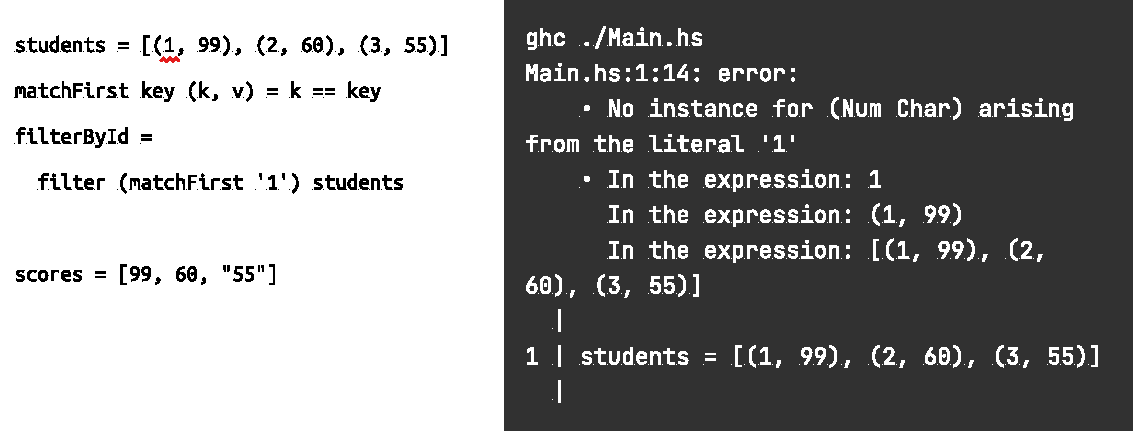
\includegraphics[width=\linewidth]{images/motivation}
    \caption{Inspecting a type error using the Haskell compiler GHC (Glasgow Haskell Compiler)}
    \label{fig:motivation}
\end{figure}

To tackle the challenges of diagnosing and resolving type errors in statically typed languages like Haskell, we introduce a novel tool: \textit{Goanna}. Goanna serves as a standalone Haskell type checker and debugging environment. Unlike conventional type-checking tools, Goanna improves error reporting by offering a comprehensive list of potential causes and suggesting accurate locations of causes. Goanna implements programming slicing and constraint programming techniques. Particularly, Goanna uses  Minimal Correction Subsets (MCS), identifies complete sets of locations that represent possible causes, setting it apart from previous type debugging systems (as detailed in Section \ref{sec:related-work}).

To further augment Goanna's capacity for type-error resolution, we introduce optimization strategies (Section~\ref{sub:optimization}) that filter out unhelpful suggestions, along with ranking heuristics (Section~\ref{sub:ranking}) that prioritize the most probable causes. Additionally, we present Goanna-IDE, an interactive programming environment for Haskell that facilitates visualization and easy navigation of Goanna's type error diagnostics.

We conducted a corpus studies on two datasets to assess Goanna's accuracy and reliability (Section \ref{sub:eval-accuracy}); while our benchmark study evaluates Goanna's performance (Section \ref{sub:eval-performance}). Results demonstrate that Goanna consistently provides accurate and reiliable error diagnostics when compare to conventional tools. Goanna shows performance constraint when diagnosing large programs containing complex type errors. However, Goanna is able to provide realtime debugging assistance when working with small to medium programs.

The main contributions of this research are:
\begin{itemize}
    \item A categorization of type errors that help reasoning about the their causes and complexity.
    \item Goanna, a Haskell type checker with advanced error reporting capabilities.
    \item Goanna-IDE, an interactive Haskell development environment that support debugging type errors using Goanna's diagnositics.
    \item A rigorous evaluation of Goanna's accuracy, reliability, and performance.
\end{itemize}

The techniques employed in Goanna, such as MUS enumeration and the ranking heuristics, are not confined to Haskell. These techniques are broadly applicable to statically typed programming languages, and Goanna is deliberately designed for adaptability across languages with similar type systems.

\section{Goanna-IDE Walkthrough} \label{walkthrough}
In this section we  demonstrate Goanna's features using some real world examples. To showcase the debugging features,  we developed Goanna-IDE, a type error debugging interface for Haskell. Goanna-IDE is designed around the pitfalls of common typecheckers and the different categories of type errors. It make extensive use of Goanna's type error diagnosis through visualization and interactivity. Goanna-IDE provides comprehensive diagnostic error messages for type errors in Haskell and allows programmers to interactively explore their options. An online demo of Goanna-IDE is available for evaluation at \cite{Fu2023-bo}. Goanna-IDE includes a file explorer, a text editor, and a debugging panel. Goanna-IDE provides the following features when type errors are encountered:

    \begin{itemize}
        \item Thoroughly detect all type errors within the codebase and allow users to inspect each type error individually via the debugging panel.
        \item Indicate the most likely causes by star indicators.
        \item Show necessary type hints in the editor panel to help reason about each possible cause.
        \item Allow users to trace type errors across multiple files.
    \end{itemize}

    \subsection{Examples of Diagnosing Type Errors with Goanna-IDE}

    For the type error in the motivating example, Goanna shows 6 possible causes of the error (see top right corner of Fig.~\ref{fig:goanna-example-1}). When focussing on the cause suggested by GHC, instead of highlighting only the literal \texttt{1}, Goanna reports all 3 literals that needed to be changed all at once if the programmer chooses to address this cause. In addition, Goanna also indicates that these integer literals need to be changed to \texttt{Char} type using the inlay type hints on line 1, largely narrowing down the potential ideal fixes. 

    \begin{figure}[ht!]
        \centering
        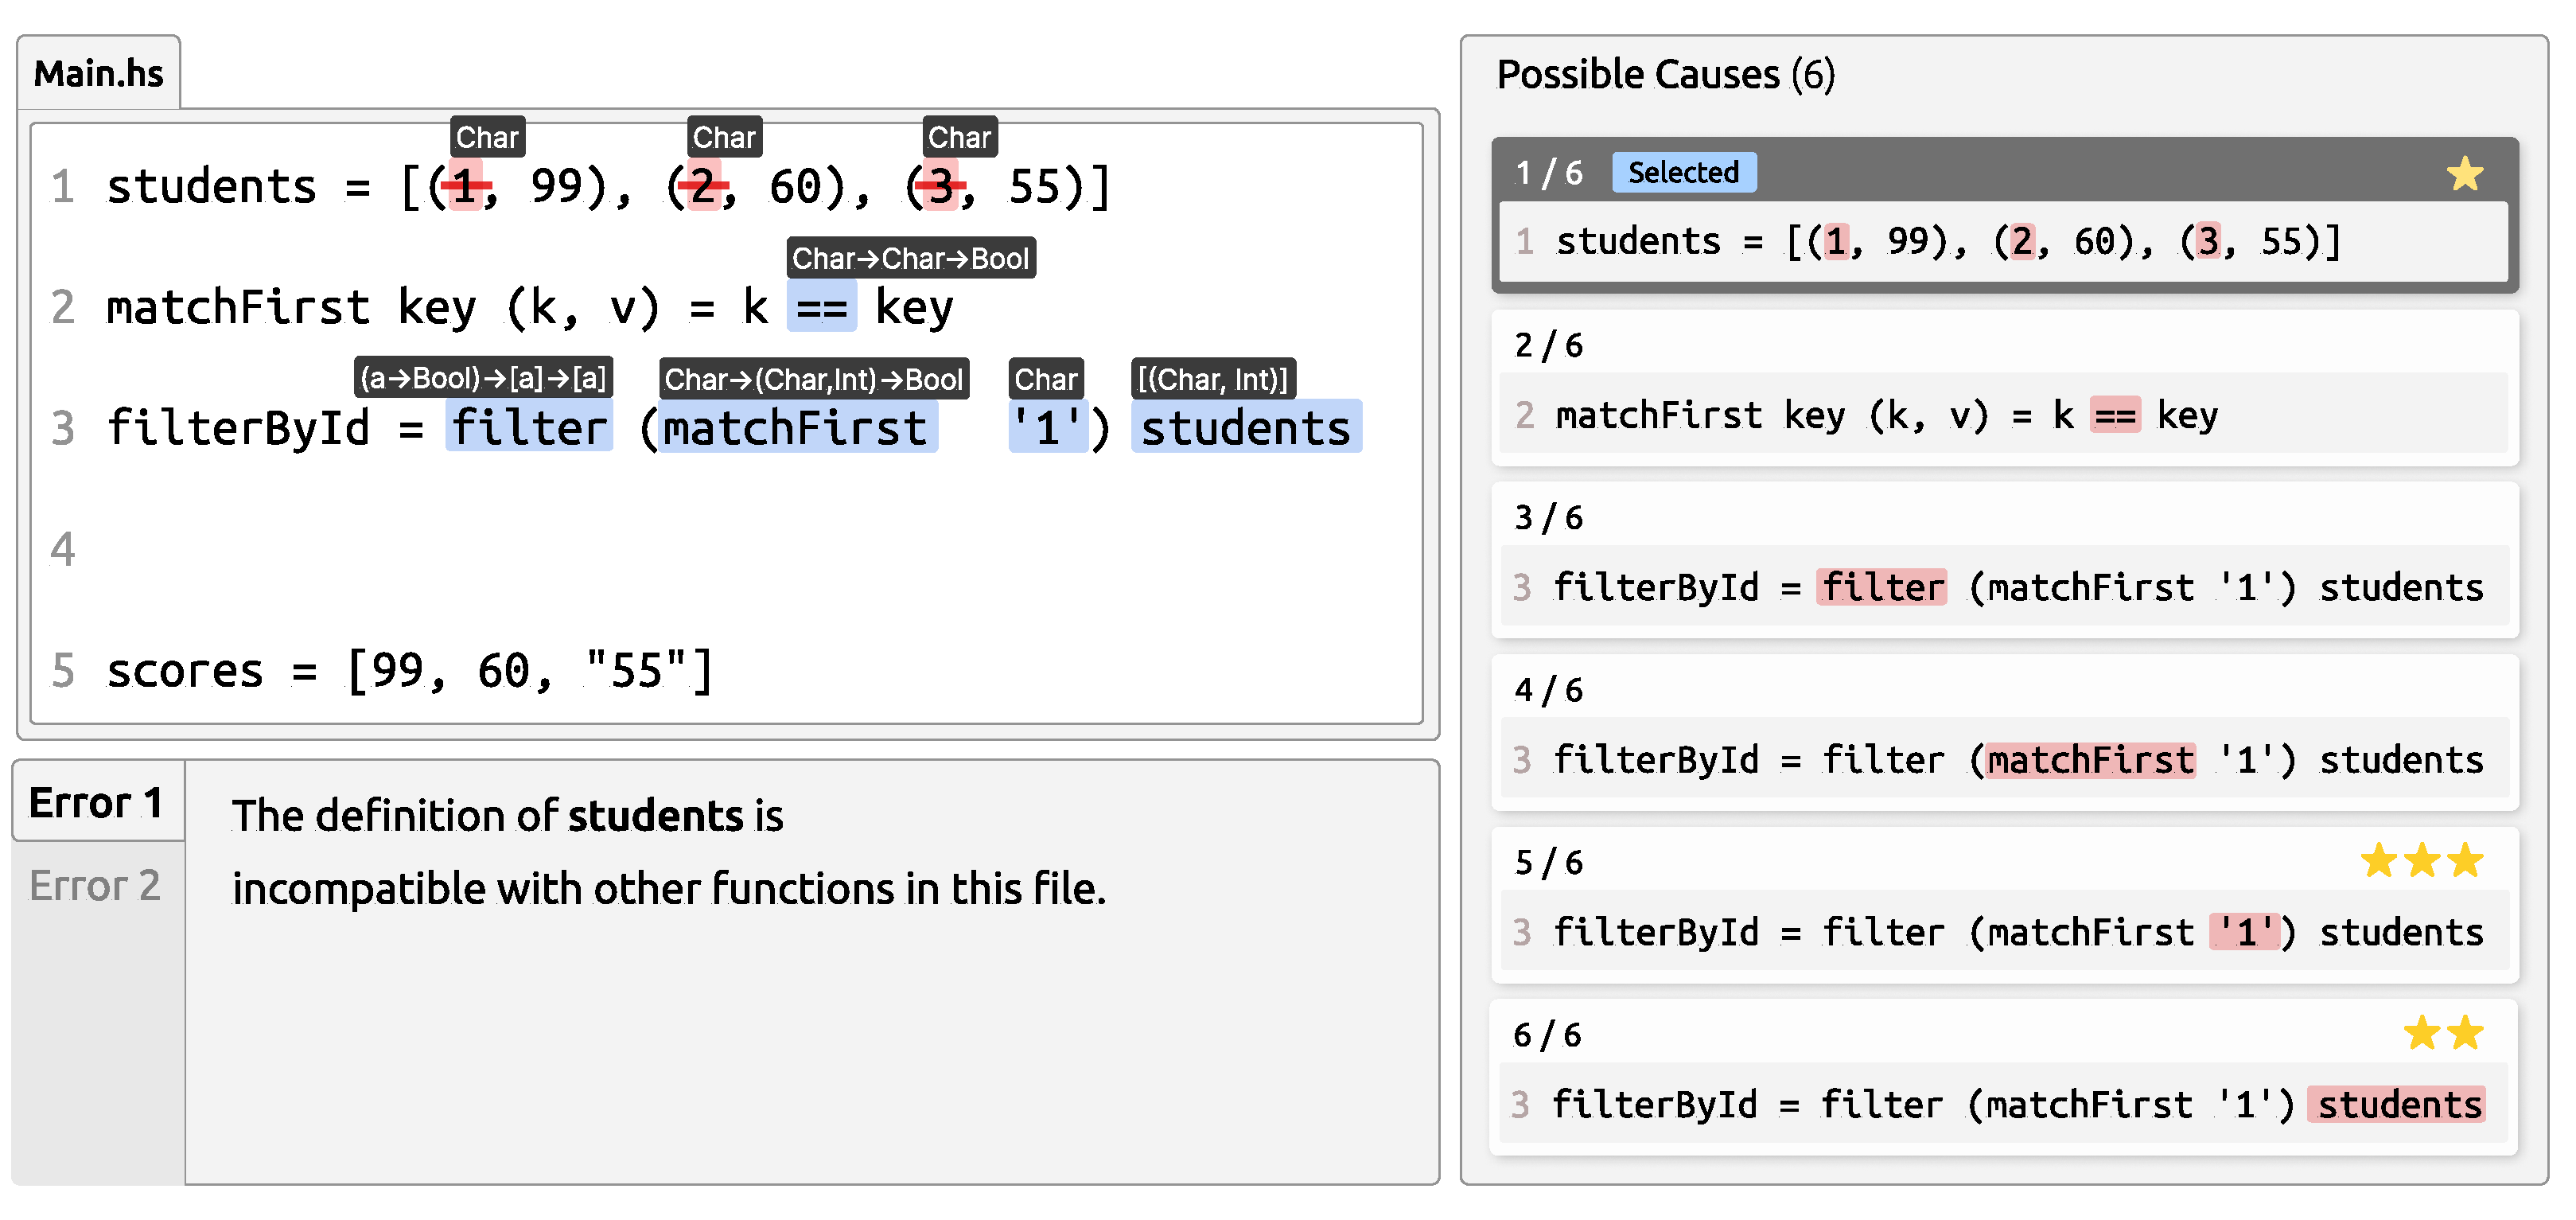
\includegraphics[width=\linewidth]{images/Goanna-Example-1}
        \caption[Goanna's showing possible causes of a type error (1)]{\textbf{Goanna's error diagnosis} Goanna shows that to fix the type error, the literals \texttt{1}, \texttt{2}, and \texttt{3} on line 1 need to be changed to Char type.}
        \label{fig:goanna-example-1}
    \end{figure}


    Note that the cause suggested by GHC is only one of the possibilities identified by Goanna. In fact, Goanna suggests that there are more likely fixes, indicated by the star symbols. The most likely fix, based on Goanna's cause heuristics (Section \ref{sub:ranking}), is the \texttt{Char} literal \texttt{'1'} on line 5, indicated by the 3 stars (Fig.~\ref{fig:goanna-example-1}).
    
    
    By clicking on the most likely cause, Goanna shows different highlights in the editor (e.g., see Fig.~\ref{fig:goanna-example-2}). Goanna reports the error is caused by the literal \texttt{'1'} and suggests changing to an integer. All the type hints are adjusted based on our new assumption. Goanna ranks all possible causes using a series of heuristics. In this case, the preference is largely influenced by how many locations are required to change to fix the error. 
    
    \begin{figure}[ht!]
        \centering
        \includegraphics[width=\linewidth]{images/goanna-example-2}
        \caption[Goanna's showing possible causes of a type error (2)]{\textbf{Goanna's error diagnosis.} Goanna shows that the type error can be fixed by changing the literal $'1'$ on line 3, which needs an \texttt{Int} type. This, according to Goanna, is the most likely cause of the type error.}
        \label{fig:goanna-example-2}
    \end{figure}


    \subsection{Identifying all type errors} \label{sub:all-errors}
    
    A key feature of Goanna is its ability to detect all type errors in the code thanks to its MCS enumeration (Subsection \ref{sub:enumeration}). This is not always the case with other tools, such as GHC, which may only report a subset of the errors present in the code or stop at the first error they encounter. Goanna, however, always thoroughly identifies all type errors in the codebase. In the example of Fig.~\ref{fig:goanna-example-1} and Fig.~\ref{fig:goanna-example-2}, Goanna discovered the two errors included in the file. Clicking on the error selector on the bottom-left will change the content of the debugging panel and text editor highlights to reflect the cause of a different error (Fig.~\ref{fig:multi-error}). 

    \begin{figure}[ht!]
        \centering
        \includegraphics[width=\linewidth]{images/goanna-multi-error}
        \caption[Selecting a different error in Goanna]{\textbf{Selecting a different error in Goanna.} Selecting a different error using Goanna's error selector. The debugging panel will show potential cause locations for the selected error. The highlights and type hints in the editor panel will focus on the selected error.}
        \label{fig:multi-error}
    \end{figure}



    \subsection{Type error grouping}  \label{sub:group}
    In addition to reporting multiple errors, Goanna also groups together type errors that might be treated as separate by other tools. Goanna uses a novel approach (section \ref{sub:grouping}) to ensure that type errors that are intuitively connected are grouped together. This means that Goanna does not overwhelm the programmer with an excessive number of redundant type errors. Instead, the programmer is presented with a concise list of errors that all can be assessed separately.

    \begin{figure}[ht]
        \centering
        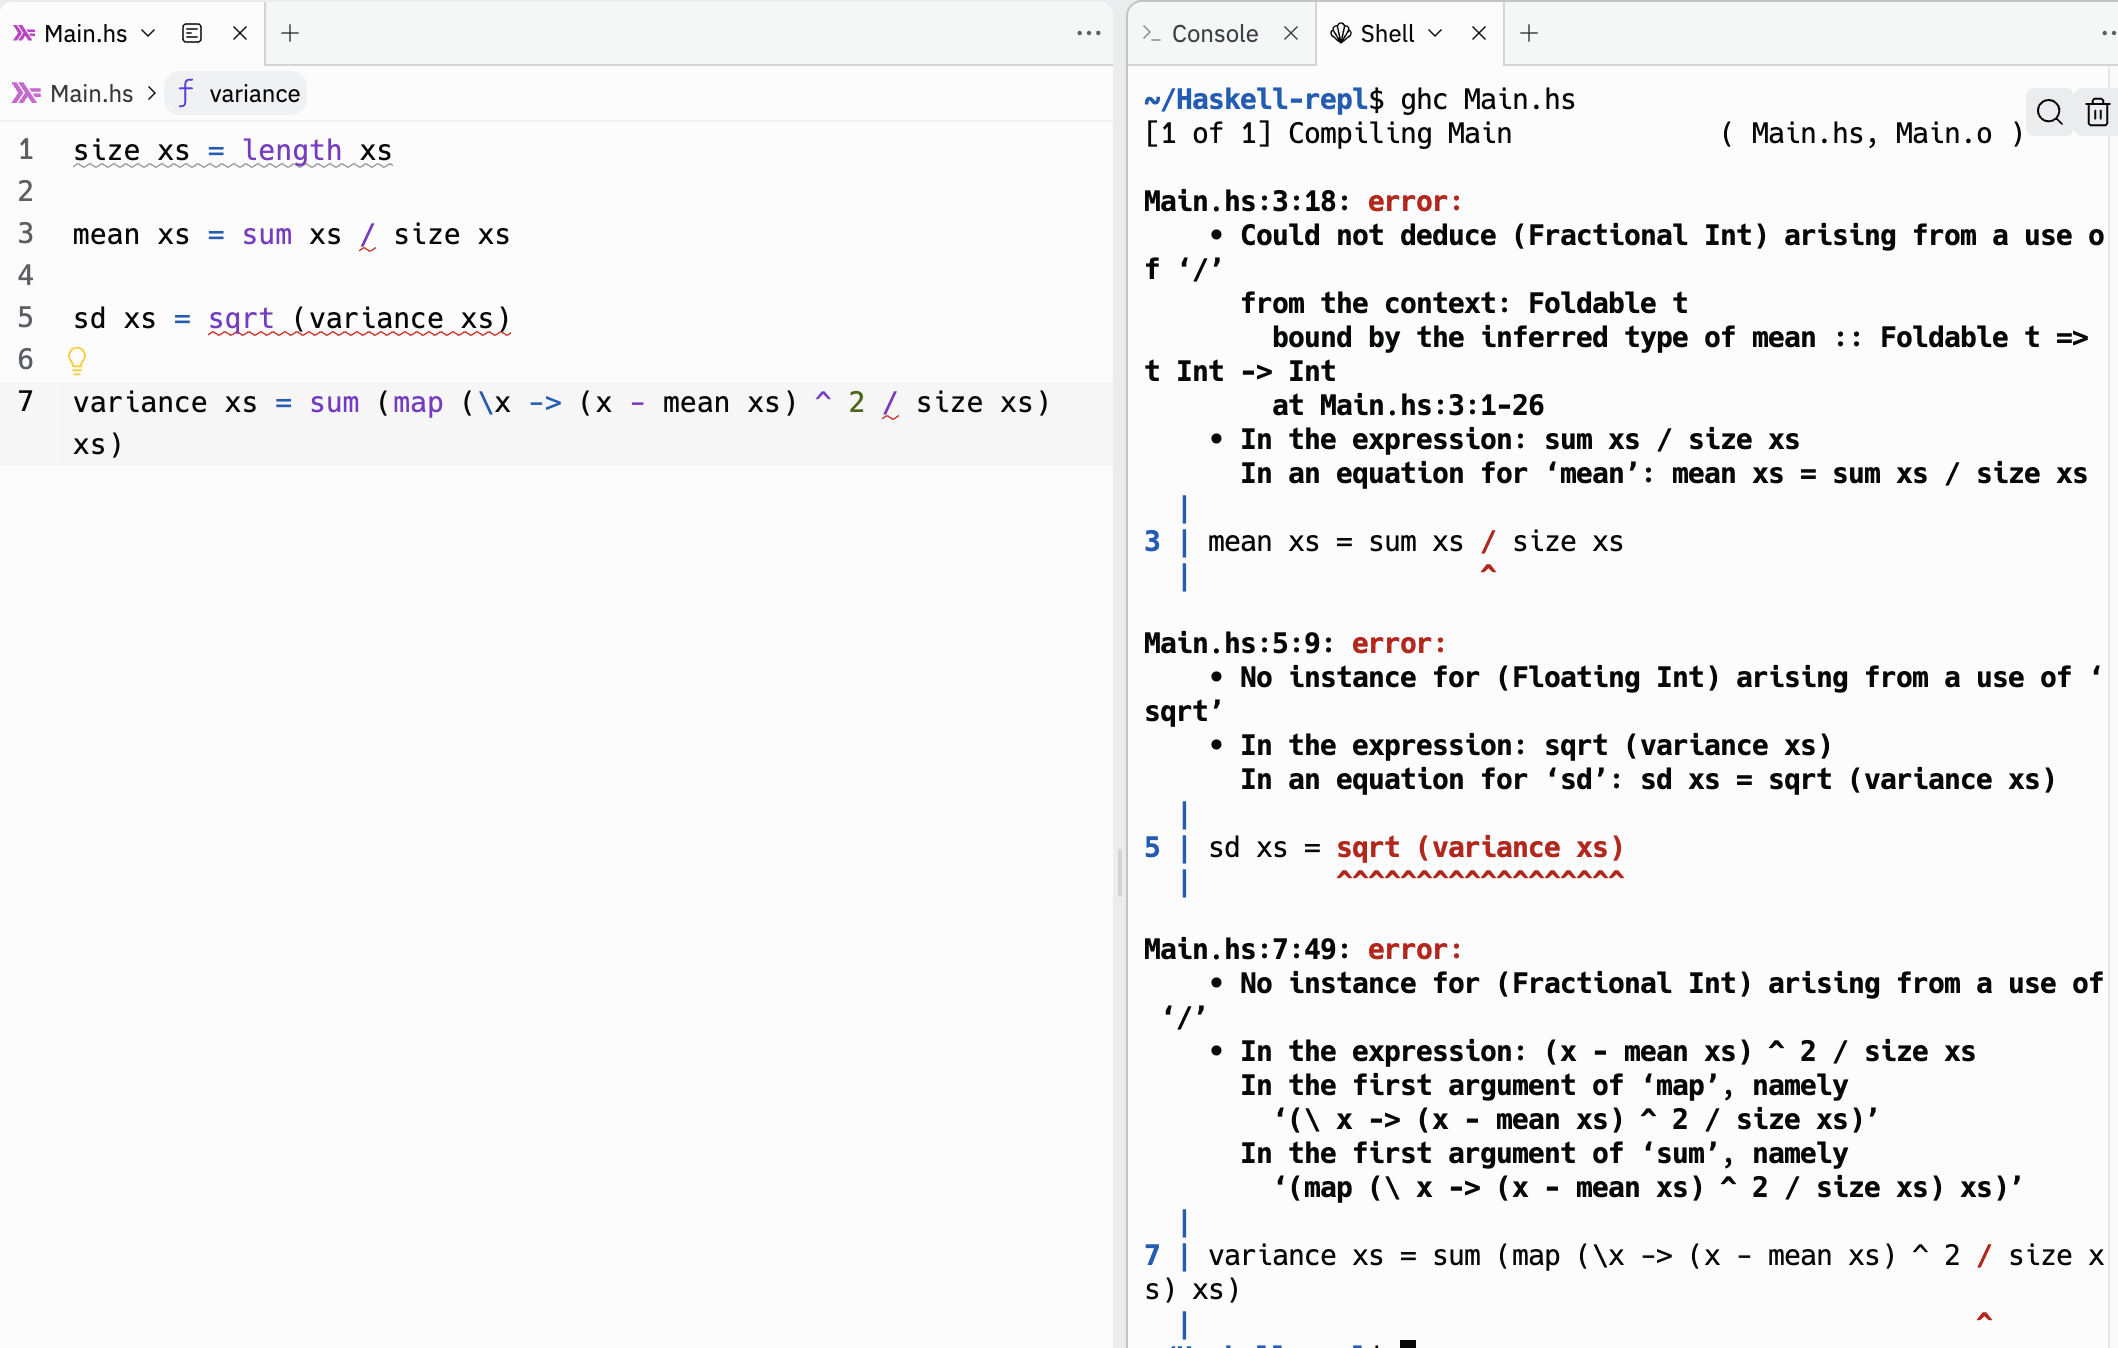
\includegraphics[width=\linewidth]{images/variance-ghc}
        \caption[Inspecting a defective Haskell Program in relation to the error messages output by the standard GHC compiler]{\textbf{Inspecting a defective Haskell Program (left) in relation to the error messages output by the standard GHC compiler (right)} -- 3 separate type errors are reported.  The editor (VS Code is used here) underlines the error locations reported in the messages, but all other contextual information must be understood from the error text.}
        \label{fig:grouping-ghc}
    \end{figure}
    
        \begin{figure}[ht!]
        \centering
        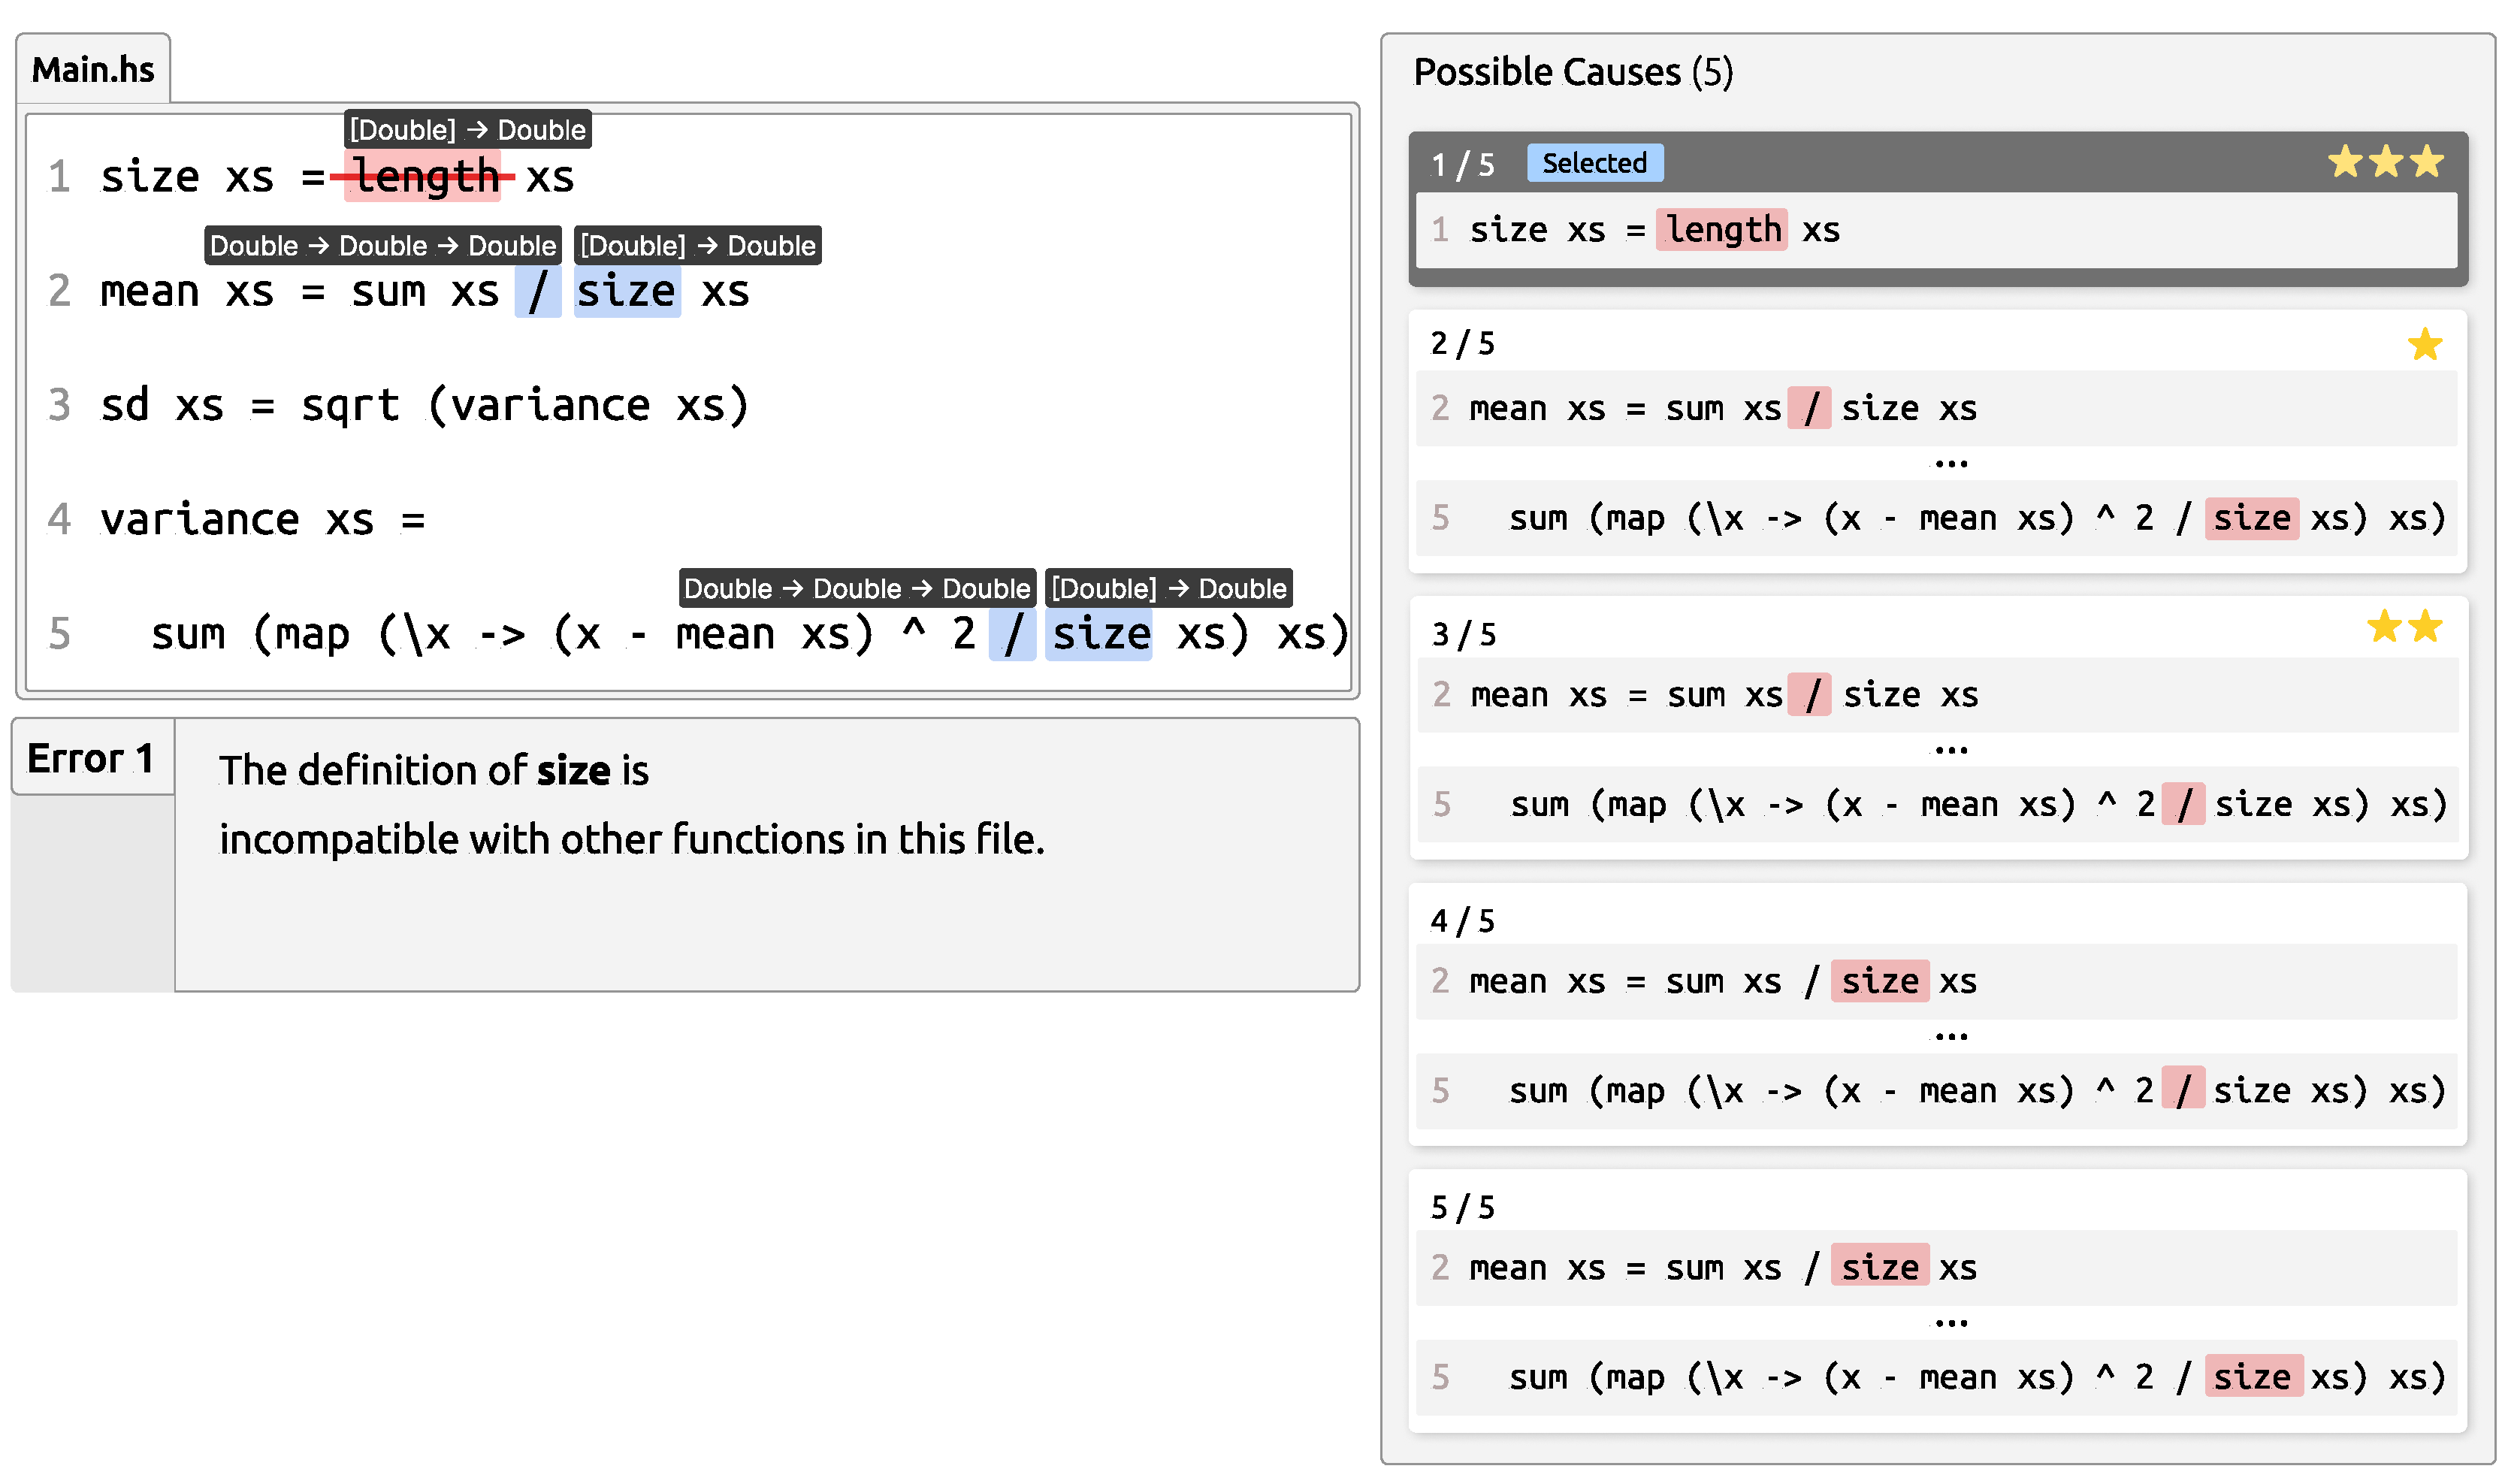
\includegraphics[width=\linewidth]{images/Goanna-Error-Grouping}
        \caption[Goanna's Error Grouping]{\textbf{Goanna's Error Grouping.} This error, although its potential offending parts appear in many declarations, is possible to fix in one place, i.e., by changing the definition of the \texttt{size} function on line 1. Therefore, Goanna reports it as a single error.}
        \label{fig:grouping-goanna}
    \end{figure}

    For instance, in Fig.~\ref{fig:grouping-ghc}, the functions \texttt{variance} and \texttt{mean} expect the final type of \texttt{size} to be a fractional value. However, the definition of \texttt{size} results in an integral value, which creates a conflict. While GHC shows three separate type errors, Goanna groups these interconnected errors into a single entity, as shown in Fig.~\ref{fig:grouping-goanna}. These errors can be addressed collectively, thereby improving the efficiency of the programmer.

    \subsection{Discovering Potential Causes} \label{sub:suggesting}
    When a type error arises, Goanna-IDE shows a list of possible causes in the debugging panel. Each possible cause consists of one or more locations in the code that require modification to rectify the type error. Clicking on a possible cause activates it. The locations are highlighted in the text editor, as well as inlay type hints suggesting the suitable type expected for that code slice. In the debugging panel, the activated cause is outlined with a red icon, while others are marked with a blue icon. 

    The causes identified by Goanna are comprehensive. Goanna will take into account potential causes in expressions, pattern matchings, type annotations, and type class constraints. Consequently, programmers will generally find the real cause by exploring Goanna's diagnosis. Unlike most Hindley-Milner~\cite{Damas1982-zw} based type inference, Goanna does not show a bias towards the unification order, thereby avoiding the left-to-right bias \cite{Chen2014-ev}. 
    
    Note that Goanna's fixes are sufficient to resolve the type error. Traditional tools often reveal a set of partial locations of a type error, leaving programmers to realize later that additional adjustments are needed for a complete resolution. Goanna, however, offers fixes that encompass a complete set of changes necessary for a resolution.


    \subsection{Assessing Likelihood of Causes} \label{sub:conciseness}
    One challenge of Goanna's ``find all causes" approach is the number of ways an error can occur can sometimes become too large to be useful in practice. Goanna employs multiple techniques to intelligently sieve the list. For the remaining list, Goanna employs a few heuristics to rank their likelihood and inform programmers which causes they consider first. 
    Goanna-IDE uses a star-based rating system to signal the ``likelihood'' of each cause. 3 stars indicating the most likely cause, 2 stars and 1 star follows. 

    \subsection{Type Hints}\label{subset:type-hints}
    In addition to suggesting which part causes that type error, Goanna-IDE explains why this is inferred by using in-situ type hints on necessary terms. The type hints are displayed as inlay decorations on top of respective fragments of source code. These type hints provide enough information for programmers to understand the type inference, and Goanna will leave out the terms that are irrelevant to the type error. Goanna's type hints are also dynamic to the selected cause. Programmers can observe how the inferred type of each term changes by changing the selected cause. Many modern programming tools use inlay type hints to support understanding, such as   Haskell Language Server~\cite{HLS-Developers2023-ot},  most often, these tools will display all type hints or none. Unlike in Goanna, these tools do not provide alternative sets of type hints for programmers to compare.
    
    \subsection{Cross-module type error debugging}\label{subsec:cross-module-type-error-debugging}
    When encountering a type error spanning across multiple modules, Goanna-IDE will group the potential causes indicated by their module and declaration block. Clicking on any possible cause location will focus the editor on the corresponding module (Fig.~\ref{fig:goanna-cross-module}). Goanna is the first tool to introduce cross-module type debugging. The way Goanna presents cross-module type errors is analogous to how run-time errors are presented in most programming languages. When encountering a run-time error, most programming environments show a call stack containing multiple file paths, and programmers can choose which file to start investigating. Often, programmers choose to start from the file authored by themselves instead of library files. Goanna uses this mental model to group potential locations that cause a type error by module and definition blocks. 
    
    \begin{figure}[ht!]
        \centering
        \includegraphics[width=\linewidth]{images/goanna-cross-module}
        \caption[Debugging a cross-module error in Goanna]{\textbf{Debugging a cross-module error in Goanna.} In this error, potential defects may appear in either module \texttt{A} and \texttt{B}. Goanna suggests 3 potential causes and fixes: 1) Change the type annotation of \texttt{x} to \texttt{[Maybe Int]} (Top). 2) Change the y variable on line 4 of module \texttt{A} to an instance of \texttt{Int}. 3) Change both the elements in the list literal in module \texttt{B} (Bottom), hence affecting the type of \texttt{y}. Clicking on each potential cause in the debugging panel results in different highlights and type hints in the editor panel.}
        \label{fig:goanna-cross-module}
    \end{figure}


    \section{Goanna Implementation} \label{sec:implementation}
    Goanna comprises 3 phases: constraint generation, MCS enumeration, and post-analysis. In the constraint generation phase, Goanna walks the abstract syntax tree and collects constraints. In the MCS enumeration phase, Goanna enumerates through all MUSes. Lastly, in the post-analysis phase, Goanna applies multiple optimization techniques to reduce the number of MCSes, group MCSes by common properties, and sort them based on heuristics.

    Goanna supports a wide and growing range of the Haskell 2010 language syntax \cite{Simon_Marlow2010-lg}. At the time of writing, fully supported features include module import/export, qualified imports, import hiding, do notation, algebraic data types, newtypes, type synonyms, type classes, operator sectioning, and range expression. Only operating in the type level, Goanna automatically support the language extensions that are not type related (RecordWildcard), and those do not extend the rules of the underlying type system (InstanceSigs). Overall Goanna support the most widely used type level extensions in Haskell and the range of supported feature is continue growing.  A detailed and updated feature coverage list can be found in \cite{Fu2023-rp}.

    \subsection{Constraint Generation} \label{sub:translation}
    Goanna uses the abstract syntax tree of the original Haskell program and translates it into a constraint program by modeling how types are defined and used. Goanna uses  portable Prolog predicates \cite{Wielemaker2011-sr} as its underlying constraint language and solver. Prolog is chosen for it is a widely used logic programming language, this helps generalize Goanna's approach to different programming languages in the future. To illustrate our constraint generation rule, we use standard Prolog notation \texttt{name/arity} (for example {\it unify/2}) here when referring to Prolog predicates, as a Prolog predicate is identified by the combination of both attributes. 
    
    For a simplified Haskell syntax shown in Fig.~\ref{fig:translation}.A, we generate a list of Prolog predicates in the language shown in Fig.~\ref{fig:translation}.B. We use 3 auxiliary functions during the constraint translation process (Fig.~\ref{fig:translation}.C) to generate Prolog variables for future unification. \texttt{fresh} makes a unique unbound Prolog variable. \texttt{var} takes a Haskell identifier name and returns a Prolog variable. Naively, this can be done by turning it to uppercase. \texttt{atom} takes a Haskell type constant/constructor name and returns a Prolog atom. Naively, this can be achieved by turning it into lowercase. We keep track of local variable names in a list $\Gamma$ containing Haskell variable names. A global variable $\mathcal{P}$ is defined to store the list of predicates being generated. To clarify, all \textcolor{blue}{parsed Haskell syntax} are in blue. All \textcolor{red}{generated Prolog syntax} are in red. 
    
    Two sets of generation rules apply to different syntax nodes and output Prolog source code. Predicate generation rules (Fig.~\ref{fig:translation}.D) take Haskell declarations as input and output Prolog predicates. For example, a Haskell function \texttt{f = 2}, Goanna may generate a predicate \texttt{\textcolor{red}{f(V, \_) <- V = int.}}
    
    Constraint generation rules (Fig.~\ref{fig:translation}.E) take a Haskell expression node or type node and a Prolog variable \texttt{V} as input and output a list of Prolog terms. These terms attempt to unify the inferred type of such node to the provided Prolog variable \texttt{V}.
    
    \begin{figure}[ht!]
        \centering
        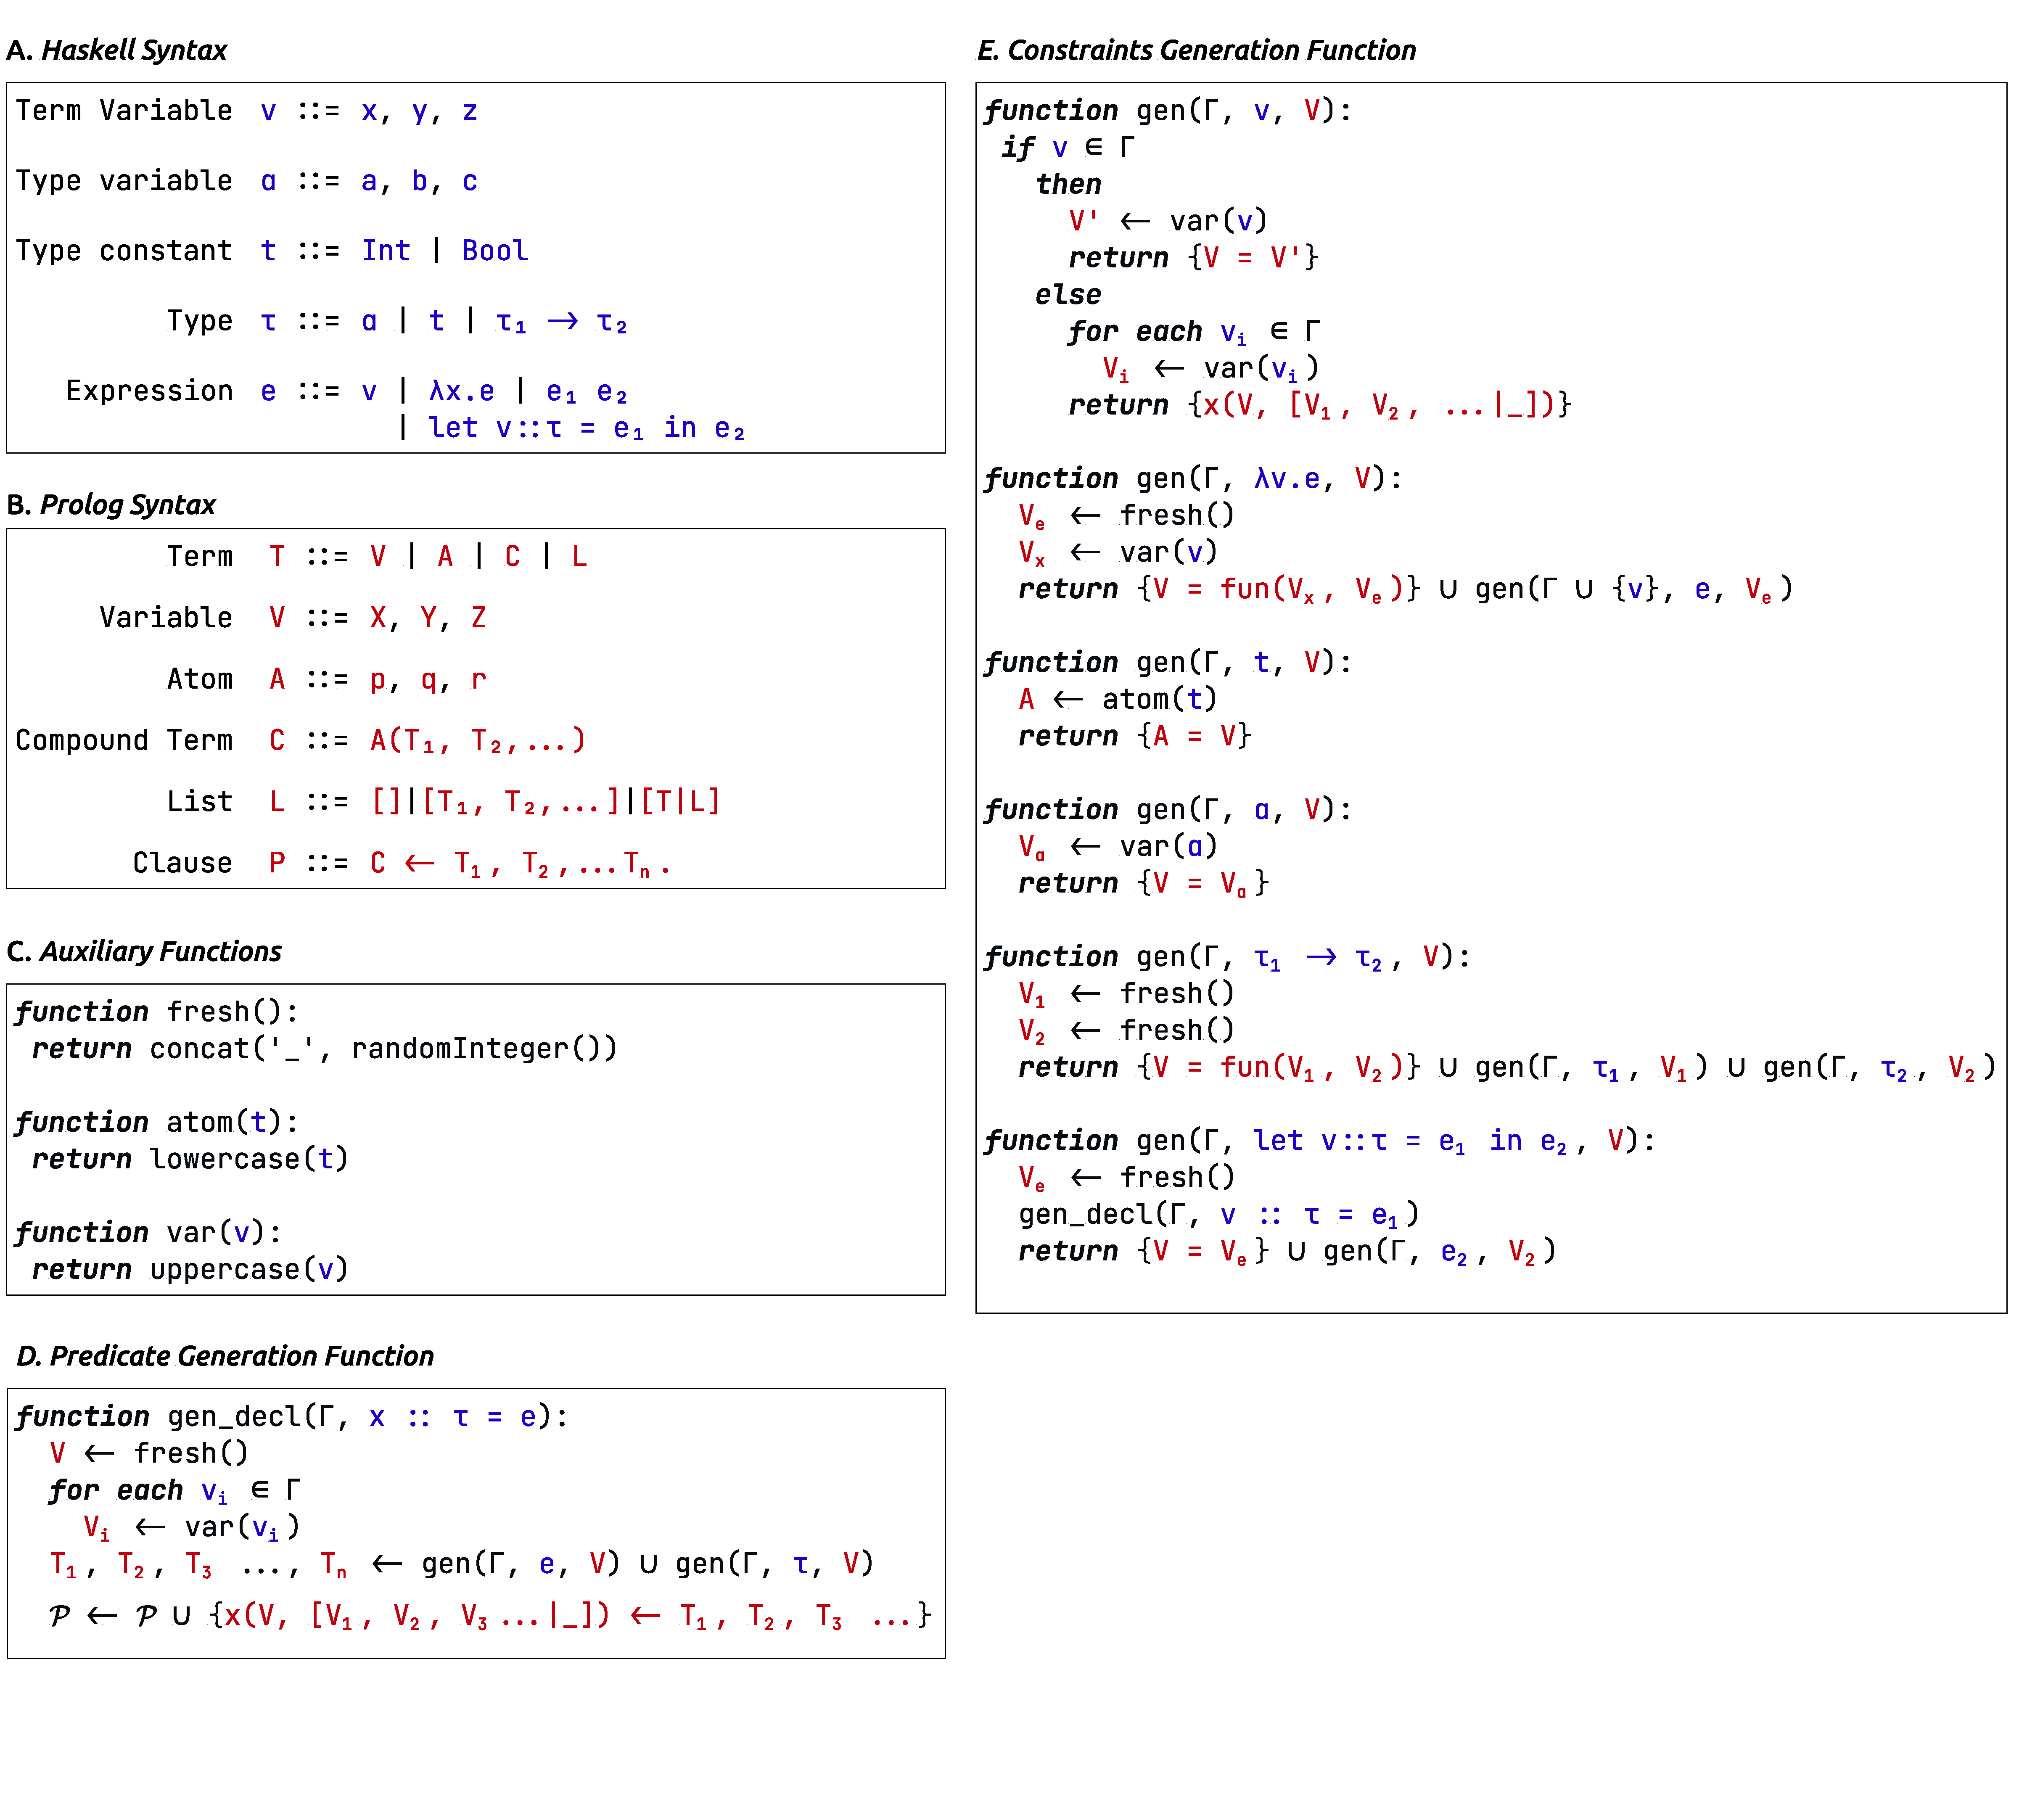
\includegraphics[width=\linewidth,trim={0 6cm 0 0},clip]{images/Generation}
        \caption{Goanna's Constraint Translation Rules (Simplified)} 
        \label{fig:translation}
    \end{figure}
    
  
    An example of such translation can be found in Fig.~\ref{fig:translation-example}. In the Haskell program (Fig.~\ref{fig:translation-example}.A), 2 functions are declared: \texttt{f} and \texttt{g}. This will generate two corresponding Prolog predicates \texttt{f/2} and \texttt{g/2}. In the actual implementation of Goanna, the generated predicates would be \texttt{f/6} and \texttt{g/6}. The extra arguments are added to perform various tasks involving syncing state, such as breaking recursive calls and collecting type class constraints. In a predefined predicate \texttt{type\_check/0}, the subgoals \texttt{f(\_,\_)} and \texttt{g(\_,\_)} are added. Executing the top-level goal \texttt{type\_check} in a Prolog environment will get a result of \texttt{false}.
    
  \begin{figure}[htb]
        \centering
    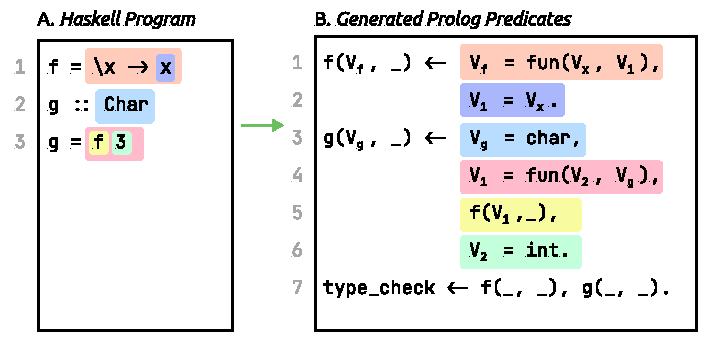
\includegraphics[width=0.7\linewidth]{images/Translation-Example}
        \caption[An example of Goanna constraint generation]{\textbf{An example of Goanna constraint generation.} For the Haskell functions \texttt{f} and \texttt{g}, Goanna generates the predicates \texttt{f/2} and \texttt{g/2}. Each subgoal of \texttt{f/2} and \texttt{g/2} is generated from a corresponding part of the Haskell program. In a predefined predicate \texttt{type\_check/0}, the subgoals \texttt{f(\_,\_)} and \texttt{g(\_,\_)} are added. Running the goal \texttt{type\_check} will return whether the program is well-typed. In this particular example, this will return \texttt{false}. We used standard Prolog notation \texttt{name/arity} here when referring to Prolog predicates, as a Prolog predicate is identified by the combination of both attribute. 
}
        \label{fig:translation-example}
    \end{figure}
    

    \subsection{MUS enumeration} \label{sub:enumeration}
    After the constraint generation phase, Goanna obtains a set of constraints $C$ derived from the source code and is able to query the feasibility of the constraint $C$ or any subsets of $C$ by calling the \texttt{solve} function. Goanna uses the MARCO algorithm \cite{Liffiton2016-xi}, an algorithms shown to enumerate MUSes efficiently. In addition to MUSes, we also obtains two other important subsets: Minimal Correction Subsets (MCSes) and Maximal Satisfiable Subsets (MSS). When we use the word subset without specifying the corresponding superset, it should be inferred as the subset of the constraint system $C$. We list these subsets obtained from MUS enumeration and give their type-theoretic interpretation. 
        
    – A minimal unsatisfiable subset (MUS) $M$ of a constraint system $C$ is a subset $M \subseteq C$ such that $M$ is unsatisfiable and $ \forall{c} \in M : M \setminus \{c\}$ is satisfiable. An MUS can be seen as a minimal explanation of the constraint system’s infeasibility. MUSes have been used extensively, mostly in combination with programming slicing, as a means to explain type errors. A MUS of type system constraints reasoning chain connecting all evidence from one location of the conflict to another. Goanna uses the set of all MUSes to group related type errors.

    – A minimal correction set (MCS) $M$ of a constraint system $C$ is a subset $M \subseteq C$ such that $C \setminus M$ is satisfiable and $\forall{S} \subset M : C \setminus S$ is unsatisfiable. MCSes are so named due to the fact that their removal from $C$ can be seen to “correct” the infeasibility. In an ill-typed program, an MCS $C$ can be seen as the ``cause" of a type error; the removal of C will result in the system being well-typed. Goanna uses MCS to represent potential causes of a type error. Each MCS contains the set of locations that need to be changed to fully resolve the type error.

    – A maximal satisfiable subset (MSS) $M$ of a constraint system $C$ is a subset $M \subseteq C$ such that M is satisfiable and $\forall{c}\ in\ C \setminus M:M\cup\{c\}$ is unsatisfiable. The definition of an MSS is symmetric to that of a MUS, with “satisfiable” and “unsatisfiable” swapped along with maximal for minimal. MCS and MSS are the complement sets of one another. In an ill-typed program, an MSS $M$ can be seen as the resulting typing environment if a type error is fixed by excluding the MCS $C - M$. Goanna uses an MSS to provide type hints for the program even when it is ill-typed.
 
     \begin{figure}[ht!]
        \centering
        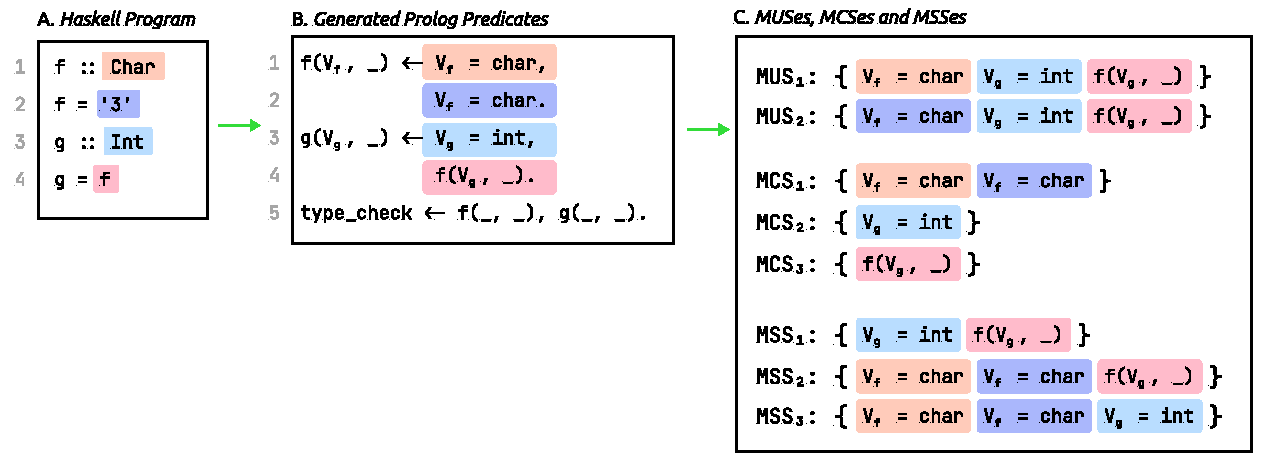
\includegraphics[width=\linewidth]{images/Enumeration-Example}
        \caption{\textbf{An example of Goanna MCS Enumeration.} From the set of constraints (B) generated from the Haskell program(A), Goanna obtained 2 MUSes, 3 MCSes, and 3 MSSes. }
        \label{fig:enumeration-example}
    \end{figure}
    
   For the example in Fig.~\ref{fig:enumeration-example}, Goanna's MUS enumeration system identifies 2 MUSes, 3 MCSes, and 3 MSSes. Following the 3 MCSes, Goanna reports 3 potential causes of the type error: the type annotation and function definition in \texttt{f} (from $MCS_1$), the type annotation alone in \texttt{g} (from $MCS_2$), and the function definition alone in \texttt{g} (from $MCS_3$). 


\subsection{Categories of Type Error} \label{sec:categories-2}

Using the formalization of MUSes and MCSes, we fomulated some patterns of type error. This fomulation addresses the challenges of reasoning about type errors and supporting intuitive explanation of these errors. From these patterns emerge four categories of type errors. And more complex type errors we see in practice can all be composed from one or more basic type errors from these four categories.

\subsubsection*{Simple Type Error}
A \textbf{simple type error} always involves two locations in the program that can not agree on a type assignments. Example like Listing \ref{lst:atomic-error} shows such an error. In the example, {\tt x} can be inferred as either {\tt Int} or {\tt Char} type based on line 1 or line 2. 

\begin{lstlisting}[language=Haskell, caption=The simplest form of type error, label={lst:atomic-error}]
  x :: Int
  x = '3'
\end{lstlisting}

In practice, type errors in this category are trivial to resolve. The two offending locations are close to each other, and they do not require special mental bookkeeping to trace back to the root cause. 

\subsubsection*{Multi-step Type Error}

\begin{figure}[hbt]
  \centering 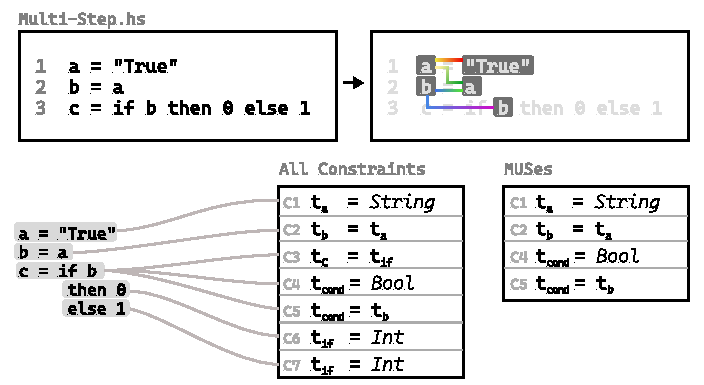
\includegraphics[width=\linewidth]{images/Multi-Step-MUS}
  \caption {A multi-step type error influenced by potential issues in the definition of \texttt{a}, \texttt{b}, or the conditional expression involving \texttt{b}. These elements are logically connected as depicted (Top Right). The analysis of the source code yields 7 constraints (Bottom Left), from which only one Minimal Unsatisfiable Subset (MUS) is identified (Bottom Right).
  }
  \label{fig:multi-step-2}
  \end{figure}

Multi-step type errors involve a sequence of logical deductions that link one conflicting location to another. When viewed as a constraint system, a multi-step type error is a type error that contains a single MUS. Relaxing any constraint within the MUS leads to a satisfiable system, implying that each location correlated to a constraint in the MUS could potentially cause the type error. For instance, in Fig.~\ref{fig:multi-step-2}, the MUS consists of the constraints $\{C1, C2, C4, C5\}$. Removing any one of the elements would allow the program to type-check successfully.

Multi-step type errors are more common in practice. They occur natually when programs develop layers of indirections or abstractions. They can cause confusion to programmers because the error can be reported at one place but the root cause is at a distant location and require tracing back and forth and mental bookkeeping. 


\subsubsection*{Multi-witness Type Error} 

\begin{figure}[hbt]
    \centering
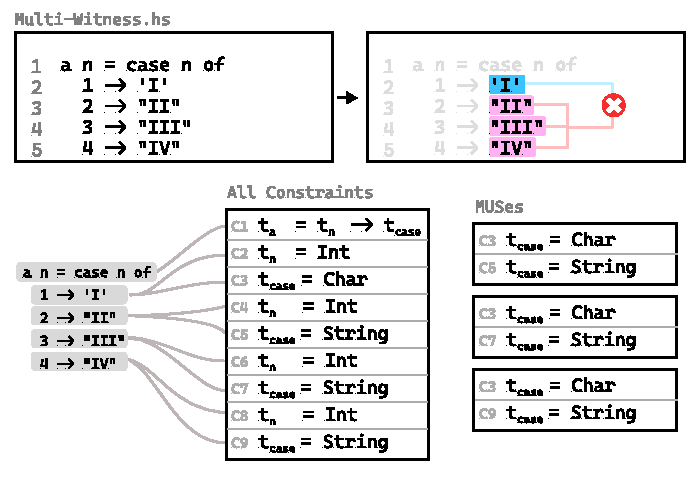
\includegraphics[width=\linewidth]{images/Multi-Witness-MUS}
  \caption{\label{fig:multi-witness-2}
    Analysis of a multi-witness type error, where the \texttt{case} expression could be interpreted as type \texttt{Char} or \texttt{String}. This scenario showcases a type conflict with three witnesses against one witness (Top Right). From the source code, 9 constraints are established (Bottom Left), resulting in 3 identified MUSes. Interestingly, all MUSes include constraint C3, suggesting its pivotal role in favoring the possibility that the \texttt{Char} type is erroneous.
  }
  \end{figure}

A multi-witness type error occurs when multiple locations (witnesses) on one side of a conflict suggest the same type assignment. When viewed as a constraint system, a multi-witness type error contains multiple MUSes. The precise number of MUSes depends on the number of witnesses at each endpoint. If a type error involves $m$ witnesses on one side and $n$ on the other, there will be a total of $m \times n$ MUSes. For example, in Fig.~\ref{fig:multi-witness-2}, there are three MUSes: $\{C3, C5\}, \{C3, C7\}, \{C3, C9\}$. It is crucial to note that the constraint C3 appears in every MUS, signaling a likely root cause.

Multi-witness type errors are also common in practice. They often occur when changes to the definition of one fragment of the program, and this fragment is referenced by multiple places. Like multi-step type errors, they too often require prorgrammers to search many locations to arrive at the correct resolution.

\subsubsection*{Multi-party Type Error}

\begin{figure}[hbt]
  \centering
  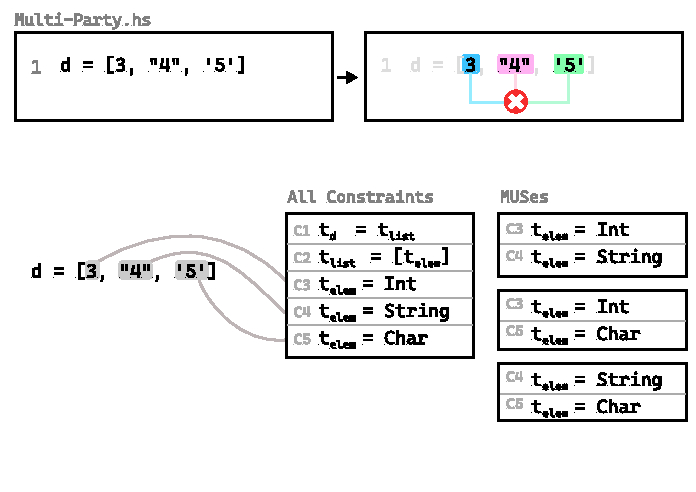
\includegraphics[width=\linewidth]{images/Multi-Party-MUS}
  \caption{\label{fig:multi-party-2} Analysis of a multi-party type error regarding the list \texttt{d}, which could alternately be typed as \texttt{[Int]}, \texttt{[String]}, or \texttt{[Char]}. The conflict is depicted as a disagreement among three parties (Top Right). An analysis based on the source code generates 5 constraints (Bottom Left), leading to 3 distinct Minimal Unsatisfiable Subsets (MUSes). Notably, this scenario differs from the multiple witness type error as no single constraint appears across all MUSes.}
  \end{figure}

  A multi-party type error features several irreconcilable type assignments stemming from different locations within the source code. Like multi-witness errors, multi-party errors contain multiple MUSes. In the example shown in Fig.~\ref{fig:multi-party-2}, there are three MUSes: $\{C3, C4\}, \{C3, C5\}, \{C4, C5\}$. Unlike the multi-witness scenario, no single element appears across all MUSes, suggesting a more complex type conflict scenario. Generally, if a multi-party type error contains $n$ parties, then there are $n (n - 1) / 2$ unique MUSes.

Multi-party type errors are not common in real life programs. They can happen when programmers mix the order of multiple arguments in function application.  
  
To We provide some strategies to improve type error diagnositics for each category:

\begin{enumerate}
  \item {
    \textbf{Simple Type Errors:}  Provide clear indication of the pair of locations associated with the error, and explain what is the logical relationship connects this pair.
  }
  
  \item {
    \textbf{Multi-step Type Errors:} To support easier trace the propogation of type error through the steps. Provide clear indication of the pair of locations associated with each step, and explain what is the logical relationship connects this them.
  }
  \item {
    \textbf{Multi-witness Type Errors:} Identify the witnesses and their associated locations on each side of the conflict. Allow programmers to quickly understand the descrepency in the number of witnesses between two sides.
  }
  \item {
    \textbf{Multi-party Type Errors:} Breaking down these errors into simpler forms to support easier understanding and resolving. Allow programmer to flexibly choose which subpart to focus on.
  }
\end{enumerate}

It is important to recognize that these categories are not mutually exclusive; a type error may exhibit characteristics from multiple categories, necessitating a combination of approaches to fully elucidate the underlying issues.

\subsection{Type Error Grouping} \label{sub:grouping}

Sometimes, it is insightful to inform programmers type inconsistencies are related to each other (caused by the same violation of typing rules) or isolated instances. To achieve this, Goanna introduce a novel feature called type error isolation. When knowing the all the MUSes, Goanna is able to analyse how many isolated type errors are there and what are the locations involved in each type error. The algorithm of performing type error isolation is as such:


	Let $U$ denote the set of all Minimal Unsatisfiable Subsets (MUSes) and $C$ the set of all Minimal Correction Sets (MCSes). We define an undirected graph $G$, where each vertex in $G$ corresponds to a minimal unsatisfiable subset $u_i \in U$, and the edges of $G$ connect pairs of MUSes $u_i$ and $u_j \in U$ if their intersection is non-empty. The set of all connected components $D$ in $G$ represents the set of all type errors. For each $d_i \in D$, let $l_i = \bigcup v_i$, where $v_i$ is the set of vertices in $d_i$. $l_i$ is the set of all constraints local to this type error. Define $C_i = \{ x \mid \forall c \in C, x = c \cap l_i \}$ as the set of all MCSes that are local to this type error.


    This can be intuitively thought of as follows: two type errors can be grouped together if they cannot be fixed independently through modifying a minimal set of locations for each. For instance, Fig.~\ref{fig:grouping-example}.A shows one connected type error, where there are two fixes available: change \texttt{0} on line 1 to a Boolean type, change the type annotation on line 3 to a \texttt{Num} instance, or change the assignment of \texttt{y} to a different expression. Choosing either one will result in both \texttt{x} and \texttt{y} being inferred to have a valid type.
    

   \begin{figure}[ht!]
        \centering
        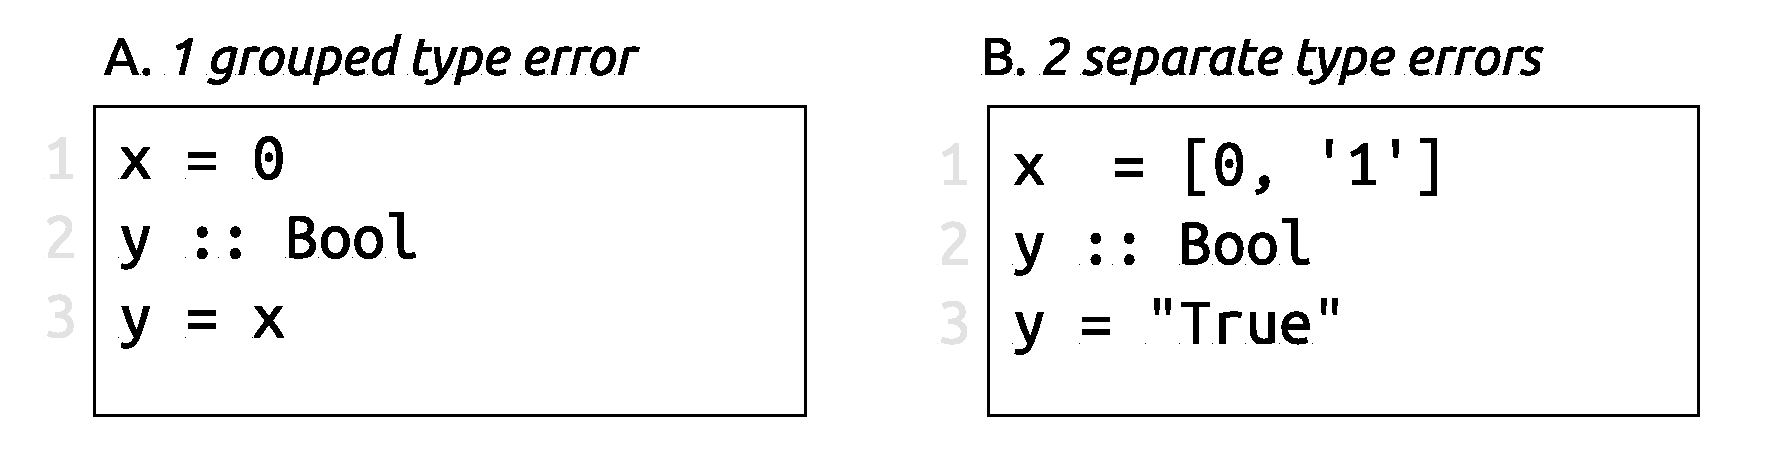
\includegraphics[width=0.8\linewidth]{images/Grouping-Example}
        \caption[Goanna's type error grouping]{\textbf{Goanna's type error grouping.} The ill-typed program on the left contains a single type error, because it can be fixed by a minimal set of syntax changes. For example, fixing it by changing the literal \texttt{0} on line 1 to \texttt{True} or \texttt{False}. This edit contains a single location, so there exists no smaller edit that can fix \texttt{x} or \texttt{y} alone. The program on the right contains two type errors because \texttt{x} or \texttt{y} can be fixed separately. For example change \texttt{0} to \texttt{'0'} on line 1 fix \texttt{x} alone. }
        \label{fig:grouping-example}
    \end{figure}


    However, in Fig.~\ref{fig:grouping-example}.B, although the ill-typed fragment is in a single function, we can fix the argument, either \texttt{0} to \texttt{'0'} or \texttt{'1'} to \texttt{1} to eliminate part of the type error. The same goes for the function's result type \texttt{x}. In this case, there are two separate type errors that should not be grouped.

	In practice, type error grouping provides a sense of the ``effective area" of a type error. Programmers are commonly bewildered by the fact that changing one place of the program causes an error in a seemingly unrelated area. When refactoring a known correct program, a programmer can change the definition of one variable, and Goanna will show all the locations that require further changes. This works because all the further changes belong to the same type error, because a single syntax change -- reverting the initial changes -- will result in the program being well-typed once more.
	
	More specifically, to Goanna, type error grouping provides an effective means to reduce the number of causes. In an ill-typed program with $m$ errors, each having $n$ potential causes, will result in $nm$ total causes. Dividing these causes into separate errors that align correctly with intuition is the most important technique to enhance Goanna's error reporting.

    \subsection{Cause Ranking} \label{sub:ranking}
     In Goanna-IDE, when a list of potential causes is on display, Goanna-IDE also shows the top ``likely" causes according to the ranking heuristics. This is very helpful because programmers will have a starting point for the investigation. We provide a set of efficient heuristics for ranking suggestions. 

    \paragraph{Number of Error Locations}
    Causes comprising fewer locations are prioritized and presented earlier in the list. For instance:
   \begin{figure}[ht!]
        \centering
        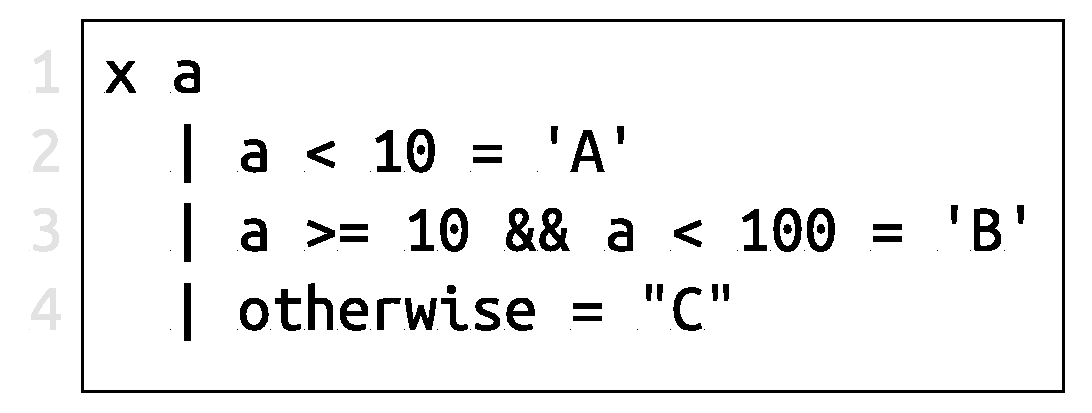
\includegraphics[width=0.5\linewidth]{images/Loc-Count}
        \caption[Goanna prefers causes with fewer error locations]{\textbf{Goanna prefers causes with fewer error locations.} In this ill-typed program, Goanna chooses to give the cause \texttt{"C"} on line 4 a higher likelihood because it contains a single location. The other cause contains 2. }
        \label{fig:loc-count}
    \end{figure}

    In the example in Fig.~\ref{fig:loc-count}, there exist two possible fixes: 1) Changing \texttt{'A'} and \texttt{'B'} to the string type, and 2) changing \texttt{"C"} to the \texttt{Char} type. As the latter fix affects only 1 location (as opposed to 2 in the former), it is assigned a higher ranking and appears earlier in the list.

    \paragraph{Change Specificity}
	Another useful heuristic is to encourage the cause whose fix will result in every surrounding term to be as concrete as possible.
	
	
   \begin{figure}[ht!]
        \centering
        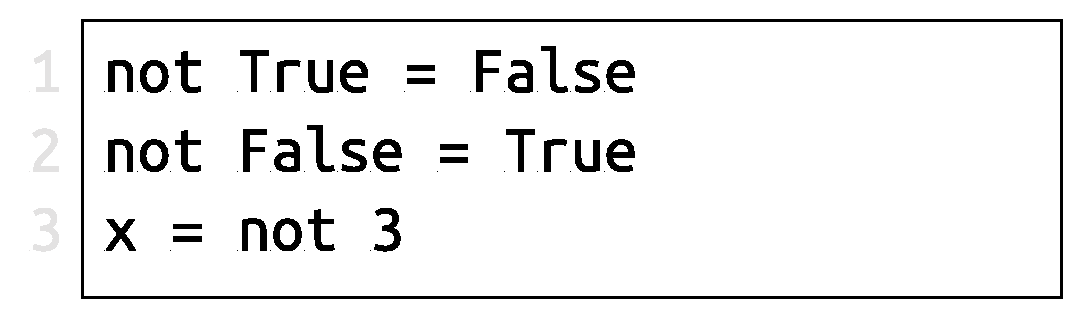
\includegraphics[width=0.5\linewidth]{images/Specificity}
        \caption[Goanna prioritize causes whose resolutions lead to more concrete type assignments]{\textbf{Goanna prioritize causes whose resolutions lead to more concrete type assignments.} In this example, change \texttt{3} will result in \texttt{x} to have type \texttt{Bool}. Alternatively, \texttt{x}'s type will be unknown after changing \texttt{not} on line 3. Goanna prefers the former.} 
        \label{fig:specificity}
    \end{figure}

    In the example in Fig.~\ref{fig:specificity}, Goanna can suggest two potential causes and fixes. First, change the integer literal \texttt{3} to a \texttt{Bool} type. Second, change the function \texttt{not} to a different function that accepts an integer as input. The second fix results in variable \texttt{x} having a less concrete type. Indeed, \texttt{x} can have any type if not limit what function to replace \texttt{not} with. Goanna prioritizes the first cause over the second. 

    
   %  \subsection{Calibration} \label{sub:optimization}
    
   %  We employ three techniques to elevate the clarity of the suggestion list: reduction of constraint count, elimination of over-fitting resolutions (solutions that are technically correct but involve making unnecessary modifications), and elimination of redundant fixes.

   %  \paragraph{Minimize Constraint Count}
   %  The number of constraints directly influences the time complexity associated with enumerating the Minimum Correction Subset (MCS). By merging multiple constraints into a singular one, we can reduce the total count of constraints and, in turn, improve the performance of enumeration. Yet, this approach requires careful application, as it could potentially lead to unsolvable situations or propose infeasible fixes, as the combined locations in the source code must either all contribute to the type error or none do. An effective application of this technique is to merge all constraints created by sub-expressions in a type signature.

   % \begin{figure}[ht!]
   %      \centering
   %      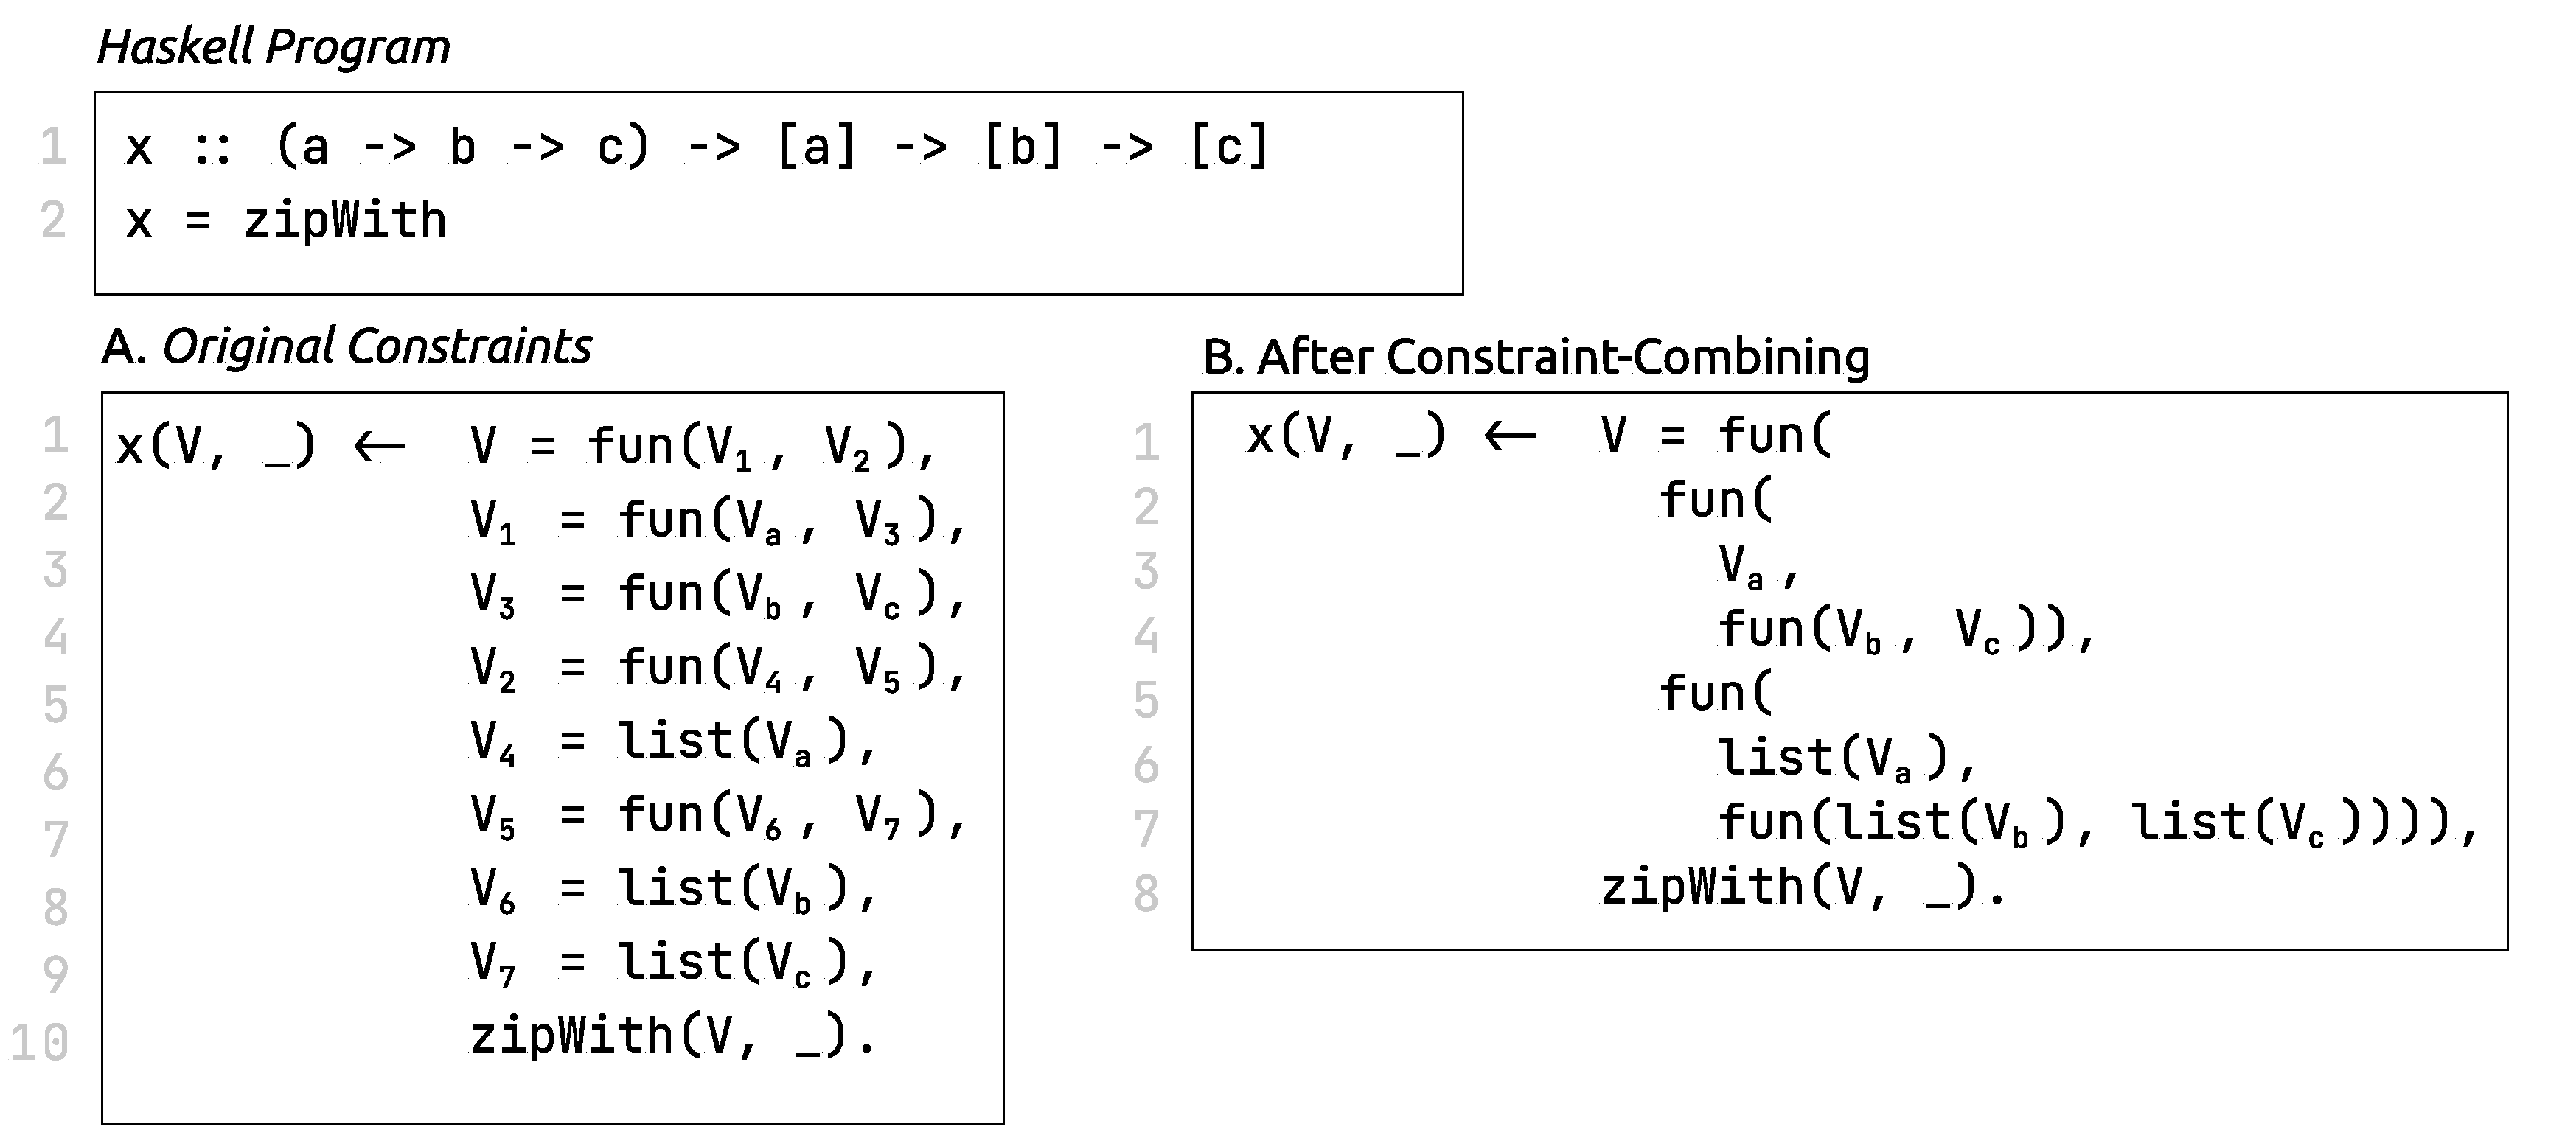
\includegraphics[width=\linewidth]{images/Combine-Constraints}
   %      \caption[Combine constraints in type signature]{\textbf{Combine constraints in type signature.} For a simple Haskell program (top),  without any optimization, Goanna generates 10 constraints (bottom left), indicated by 10 subgoals in the predicate. By combining the constraints in the type signature, Goanna produces 2 constraints (bottom right).}
   %      \label{fig:combine-constraints}
   %  \end{figure}

   %  Consider the example in Fig.~\ref{fig:combine-constraints}. Without optimization, this code would spawn 10 constraints. However, applying this optimization can achieve an equivalent outcome with merely 2 constraints. Notably, this optimization forfeits the capability to suggest fixes for sub-expressions within a type signature, a decision that warrants some consideration but, in our experience, often leads to clearer error localizations.

   %  \paragraph{Elimination of Over-Fitting Resolutions.}
   %  Over-fitting often refers to a situation where error correction tools provide solutions that are technically correct but involve making unnecessary modifications. In Goanna, every syntax node in the source code generates one or more constraints. This includes structural nodes such as function applications and let expressions. However, very often, suggesting that the user should modify the entire function application expression is not particularly instructive when changing one of the arguments fixes the type error as well. Disabling suggestions for over-fitting solutions improves the clarity of the suggestion list and enhances the speed of MCS enumeration.
   

   %  \paragraph{Elimination of Redundant Causes.}
   %  Goanna iterates over the possible causes and removes the ones that fail to deliver new insights. If all locations in a cause suggestion have already been covered in preceding suggestions, subsequent suggestions that merely rearrange these locations in different combinations can be omitted.
    
   % \begin{figure}[ht!]
   %      \centering
   %      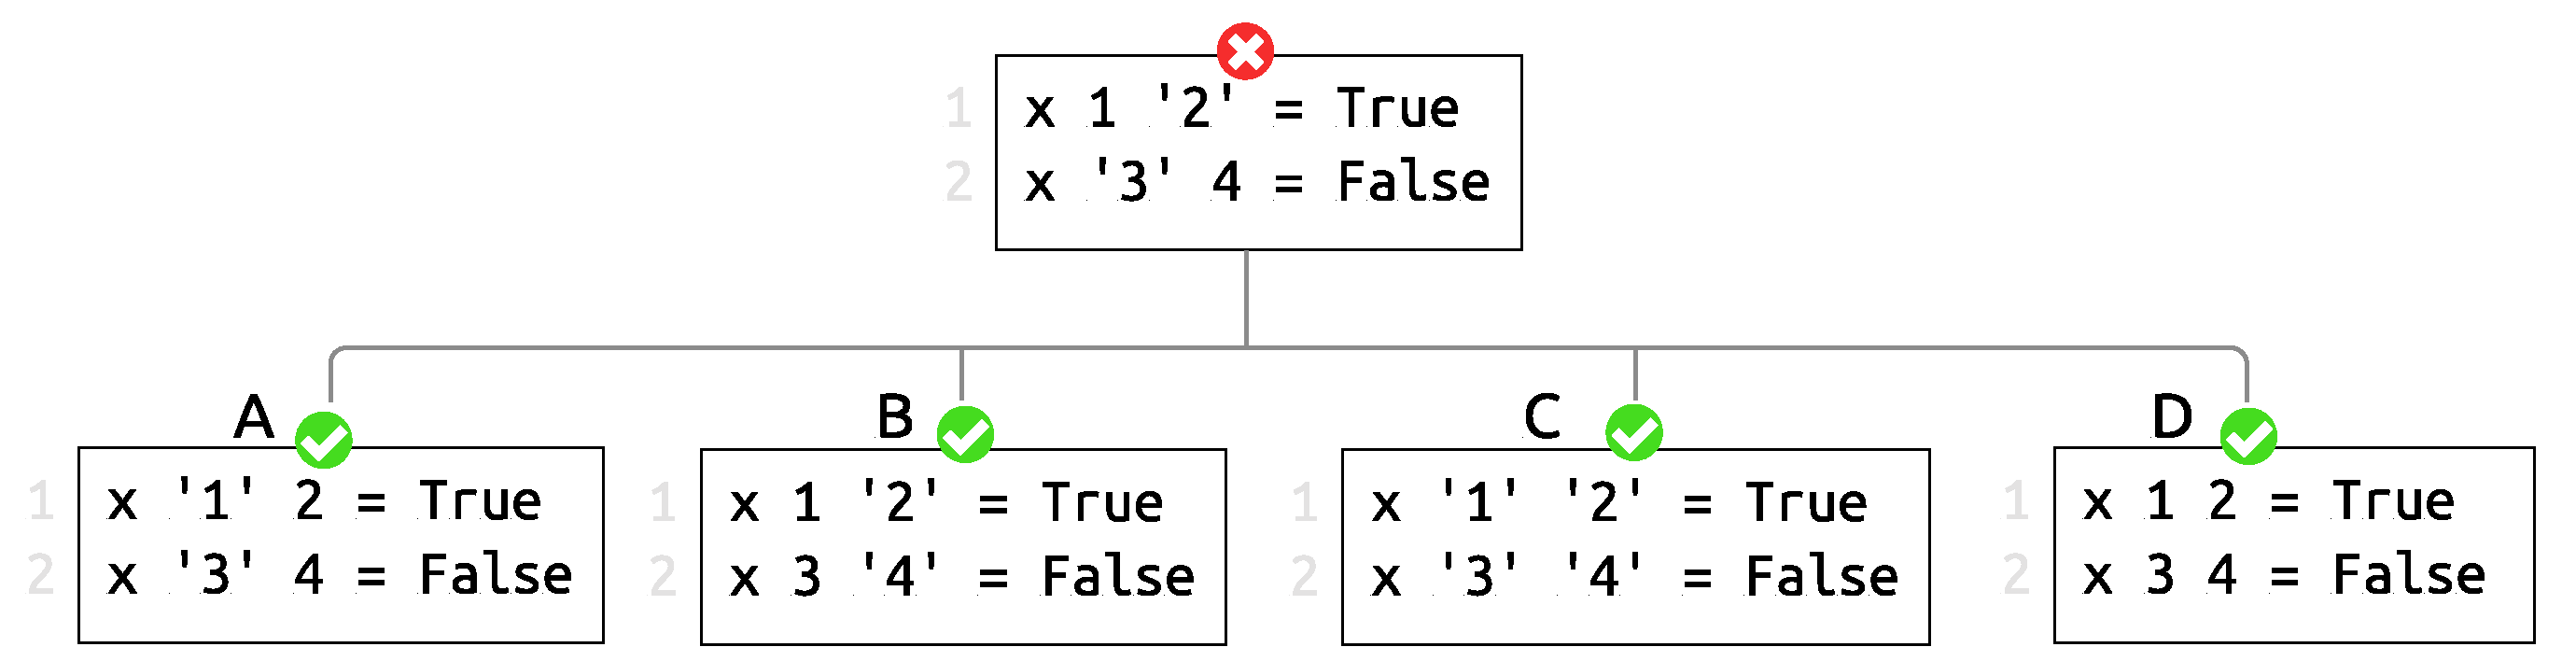
\includegraphics[width=0.9\linewidth]{images/Reduction-Example}
   %      \caption[The number of potential causes can grow exponentially]{\textbf{The number of potential causes can grow exponentially.} In the ill-typed Haskell program (Top), there are 4 different ways (Bottom) to fix the type error. It is not hard to see this growth is exponential, and showing all the alternatives is not helpful.}
   %      \label{fig:reduction-example}
   %  \end{figure}
    
   %  Consider the example in Fig.~\ref{fig:reduction-example}. Without knowing the true intention of the programmer, Goanna can provide four ways to fix the issue shown at the bottom. However, closer inspection reveals that after the first two suggestions, we no longer unearth new insights. Therefore, they can be removed to enhance the clarity of the suggestion list. 
   %  Note that this can remove the correct answer (say D), but if the programmer uses part of the (A) to make the fix, the revised type error will include the correct fix. 
    
   %  Removing superfluous MCS-based suggestions that recycle different permutations of the same set of locations is an instantiation of the Set Cover Problem (SCP). The problem can be rephrased as finding the minimal number of MCSes that cover all the potential locations that could cause the type error. Many approaches solve the SCP \cite{Caprara2000-vw}, including eager algorithms, linear programming, and heuristic-based algorithms. Generally, we found all of these approaches find the minimal cover of type errors efficiently. Goanna uses the OR-tools \cite{Google_Developers_undated-ew} for this task.
       
\section{Evaluation} \label{sec:evaluation}

In evaluating Goanna as a type error debugging environment, we aim to address the following key research questions:

\begin{enumerate}
    \item \textbf{RQ1} Can Goanna identify type errors more accurately compared to traditional tools?
    \item \textbf{RQ2} How long does it take Goanna to provide these type error diagnoses?
\end{enumerate}

To answer {\bf RQ1}, we conducted a corpus study on defective Haskell programs compiled from online channels and research papers. For {\bf RQ2}, we performed benchmarks using generated Haskell programs with controlled properties.

\subsection{The Datasets} \label{sub:dataset}

We compiled two datasets of defective Haskell programs (N=153) for running the evaluation. The first dataset (N=86), named \texttt{Haskell Community}, was sourced from Haskell online discussions forums, each containing one or more type errors. These include StackOverflow, Reddit, and Discord (Table. \ref{tab:haskell-community}),  top communications channels for Haskell users based on a research survey \cite{Fausak2022-zf}. We focused on discussions where authors encountered type errors and sought help, and including only those with accepted solutions by the original authors. The second dataset (N=67), called \textit{Haskell Academic}, was compiled from peer-reviewed research papers (Table. \ref{tab:haskell-research}) that are related to Haskell type errors.

Program lengths ranged from 1 to 64 lines of code (mean=20, median=20). These programs covered a variety of themes, including basic syntax (14 files), lists (28 files), tuples (5 files), algebraic data types (22 files), higher-order functions (17 files), monadic operations and do notation (9 files), type classes (6 files), and built-in/library functions (24 files). This thematic distribution aligns with the different causes of type errors from Tirronen's study \cite{Tirronen2015-nr}.

\begin{table}
\centering
\begin{tabular}{|p{5cm}|c|c|c|}
    \hline
    \textbf{Paper} & \textbf{Type} & \textbf{Tool} & \textbf{Programs} \\ \hline

  \raggedright
    How Type Errors Were Fixed and What Students Did? &
    Empirical Study &
    &
    14  \\ \hline

  \raggedright
    Helium: for Learning Haskell &
    System/Tool &
    Helium &
    7 \\ \hline

  \raggedright
    Diagnosing Haskell Type Errors &
    System/Tool &
    SHErrLoc &
    1 \\ \hline

  \raggedright
    SHErrLoc: A Static Holistic Error Location &
    System/Tool &
    SHErrLoc &
    1 \\ \hline

  \raggedright
    Counterfactual Typing for Debugging Type Errors &
    System/Tool &
    Counterfactual Typing &
    2 \\ \hline
  
  \raggedright
    Understanding Beginners' Mistakes with Haskell &
    Empirical Study &
    &
    2 \\ \hline
  
  \raggedright
    Learning to Blame: Localizing Novice Type Errors with Data-driven Diagnosis &
    System/Tool &
    Nate &
    5 \\ \hline

  \raggedright
    Type Debugging with Counterfactual Type Error Messages Using an Existing Type Checker &
    &
    &
    1 \\ \hline

  \raggedright
    Improving Type Error Messages in OCaml &
    &
    &
    5 \\ \hline

  \raggedright
    Type Error Slicing in Implicitly Typed Higher-Order Languages &
    System/Tool &
    Type Error Slicing &
    1 \\ \hline

  \raggedright
    Getting into the Flow &
    System/Tool &
    &
    1 \\ \hline

  \raggedright
    Learning User-friendly Type-error Messages &
    System/Tool &
    LearnHaskell &
    3 \\ \hline

  \raggedright
    ChameleonIDE: Untangling Type Errors Through Interactive Visualization and Exploration &
    System/Tool &
    ChameleonIDE &
    4 \\ \hline

  \raggedright
    Investigating Compilation Errors of Students Learning Haskell &
    Empirical Study &
    &
    5 \\ \hline

  \raggedright
    The Chameleon Type Debugger (Tool Demonstration) &
    System/Tool &
    Chameleon &
    6 \\ \hline

  \raggedright
    Proofs about a Folklore Let-Polymorphic Type Inference Algorithm &
    System/Tool &
    Algorithm M &
    2 \\ \hline

  \raggedright
    Interactive Type Debugging in Haskell &
    System/Tool &
    Chameleon &
    2 \\ \hline

  \raggedright
    Exploiting Diversity in Type Checkers for Better Error Messages &
    System/Tool &
    Lazy Typing &
    1 \\ \hline

  \raggedright
    Improving Type Error Diagnosis &
    System/Tool &
    &
    3 \\ \hline

  \raggedright
    Searching for Type-Error Messages &
    System/Tool &
    SEMINAL &
    1 \\ \hline

  \raggedright
    Finding Minimum Type Error Sources &
    System/Tool &
    MaxSMT Based Tool &
    1 \\ \hline

\end{tabular}
\caption{Summary of Studies and Tools in Haskell Research}
\label{tab:haskell-research}
\end{table}

\begin{table}
\centering
\begin{tabular}{|c|c|}
    \hline
    \textbf{Source} & \textbf{Programs} \\ \hline
    StackOverflow & 32 \\ \hline
    Haskell on Reddit & 20 \\ \hline
    Haskell Discord & 34 \\ \hline
\end{tabular}
\caption{Distribution of Programs from Online Haskell Communities}
\label{tab:haskell-community}
\end{table}

\subsection{Accuracy and Reliability} \label{sub:eval-accuracy}

We define accuracy in type error diagnosis as whether the reported error aligns with the user's real intention. Similarly, reliability indicates whether the type error can be resolved by making suitable changes to the reported location. An error diagnosis can be reliable but accurate. For each defective program in our datasets, we compare Goanna's error diagnosis against the oracle answer to measure the overall accuracy. A diagnosis is deemed accurate if its suggested fix matches the accepted answer in all of its reported locations. It is considered reliable if the type error can be resolved when the reported locations are changed to values of the bottom type (\textit{undefined} in Haskell).

We compared Goanna with the Glasgow Haskell Compiler (GHC) version 9.4 \cite{Gamari_undated-zu} and Helium \cite{Hage2023-kk} version 1.8. GHC is the most widely used Haskell compiler, known for its comprehensive capabilities and efficiency. Helium is another well-regarded Haskell compiler, noted for producing high-quality error messages \cite{Heeren2003-kd}. Because Goanna suggests multiple potential causes, and it technically always include the accurate cause in its diagnositics. Therefore, in this comparason, we only included two variations: Goanna-1 (considering only the top suggestion) and Goanna-3 (considering the top three suggestions).

\begin{figure}[ht!]
    \centering
    \begin{subfigure}{0.49\linewidth}
        \centering
        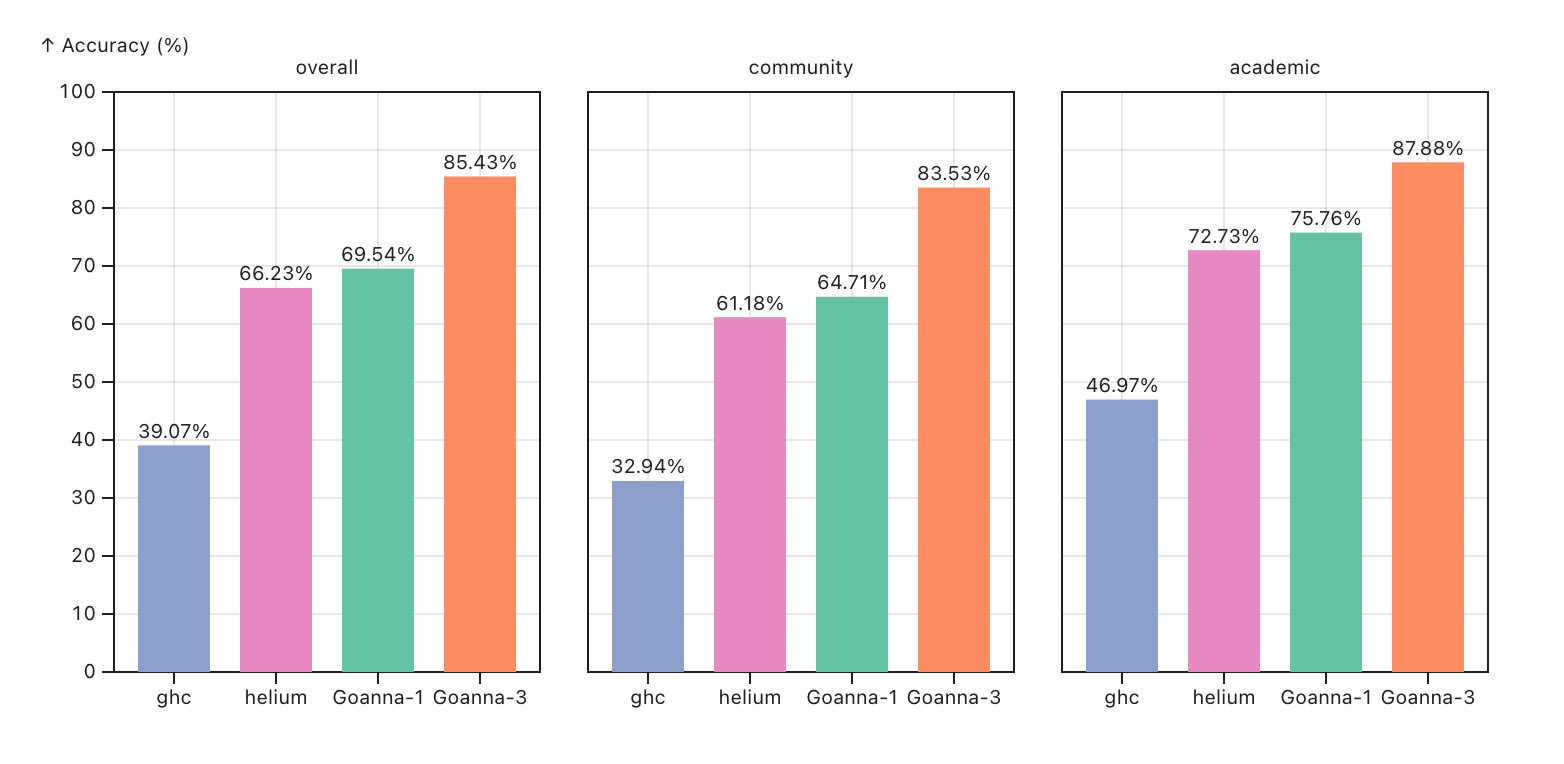
\includegraphics[width=\linewidth]{images/accuracy.png}
        \caption{Percentage of Diagnoses Matching Accepted Answers} 
        \label{fig:accuracy}
    \end{subfigure}
    \hfill
    \begin{subfigure}{0.49\linewidth}
        \centering
        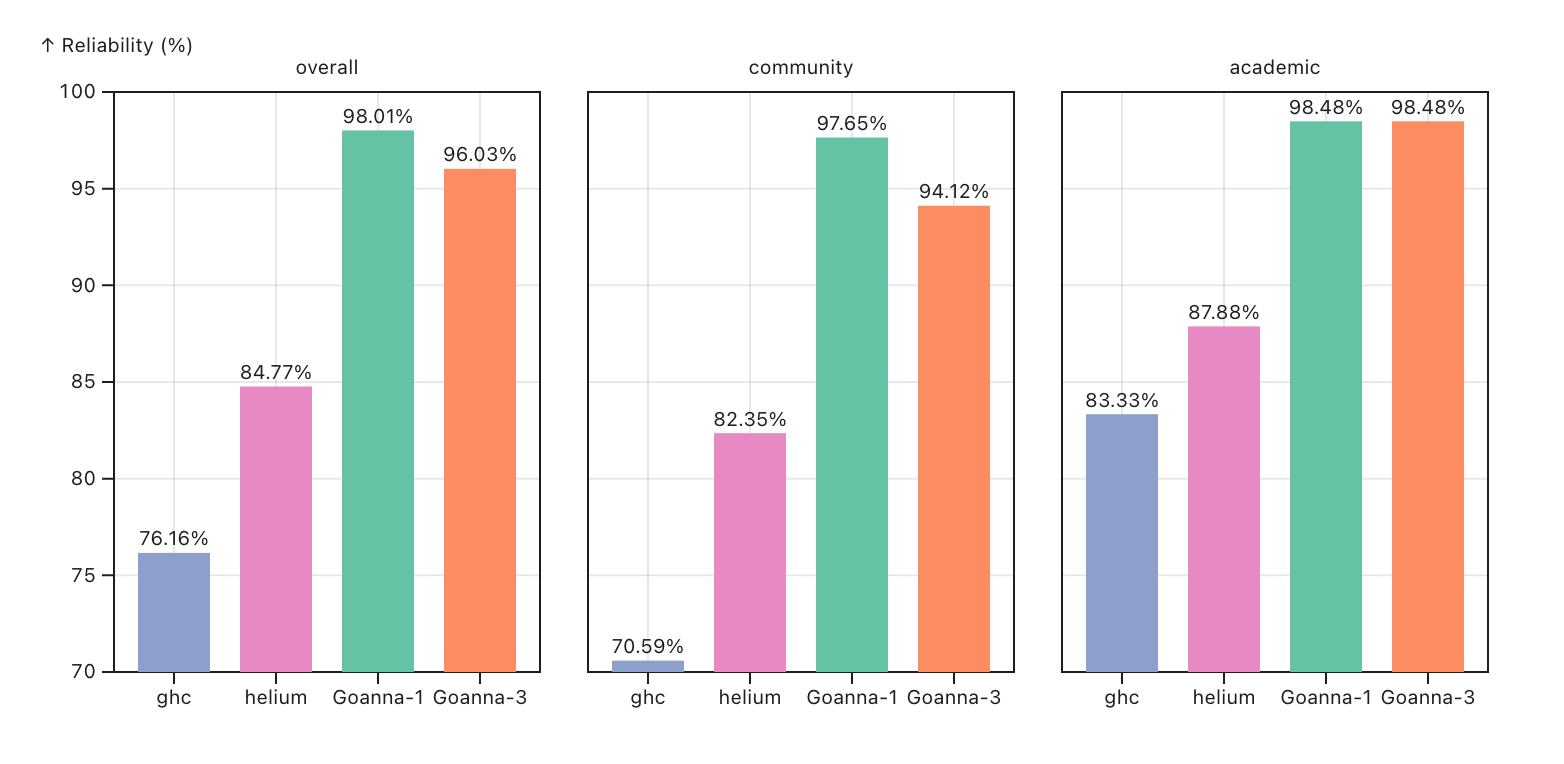
\includegraphics[width=\linewidth]{images/Reliability.png}
        \caption{Reliability of Goanna} 
        \label{fig:reliability}
    \end{subfigure}
    \caption{Comparison of Accuracy and Reliability}
\end{figure}

\textbf{Accuracy:} As seen in Fig.~\ref{fig:accuracy}, GHC's accuracy is the lowest among the tools. Goanna-1 outperforms both GHC and Helium with an accuracy of 69.54\%. \textbf{Goanna-3 achieves the highest accuracy at 85.43\%}, maintaining a consistent level across both the \textit{Haskell Academic} and \textit{Haskell Community} datasets, while other tools see drops in accuracy in \textit{Haskell Community}. For all errors in the datasets, there were no disagreements among the tools regarding the presence of errors; thus, Goanna did not miss any errors identified by other tools, nor falsely dentified a well-typed program as defective.

\textbf{Reliability:} As shown in Fig.~\ref{fig:reliability}, GHC is the least reliable (84.55\%), while Helium has modestly better reliability (88.20\%). Goanna-1 and Goanna-3 both achieve the highest reliability (100\%). GHC and Helium are unreliable when multi-witness type errors and multi-party type errors occurs. Both of these tools report only a single location. 

\subsection{Performance} \label{sub:eval-performance}
Goanna's high accuracy and reliability comes at the tradeoff in its computational complexity. As we can see in Fig. Fig.~\ref{fig:performance}, when  measuring the time required to generate full type error diagnoses on our datasets, Goanna is slower than other tools: GHC (mean=0.09s, median=0.09s), Helium (mean=0.31s, median=0.31s), and Goanna (mean=0.50s, median=0.42s). Additionally, Goanna exhibits a larger variation in performance. Since Goanna continues until all causes are detected and ranked, there is no distinction between Goanna-1 and Goanna-3 in terms of performance.

\begin{figure}[ht!]
    \centering
    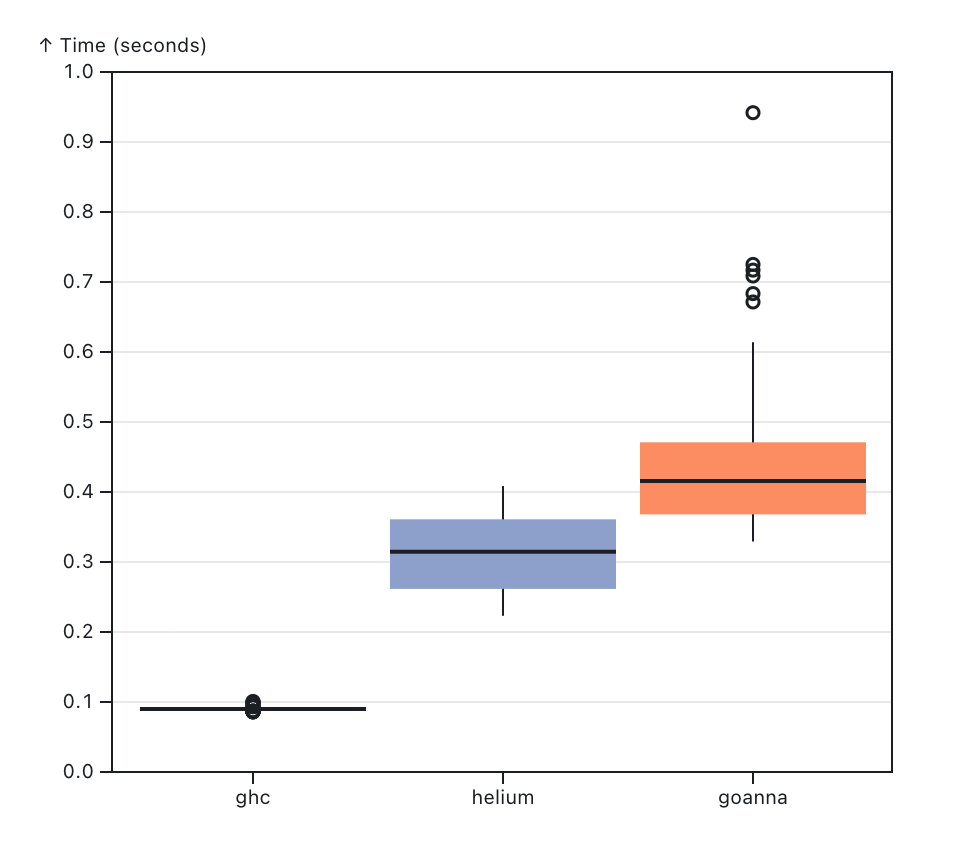
\includegraphics[width=0.7\linewidth]{images/performance-overall.png}
    \caption{Performance Comparison}
    \label{fig:performance}
\end{figure}

The computational cost of Goanna lies in Minimal Unsatisfiable Subset (MUS) enumeration, which is constrained by two main factors: (1) the cost of finding a single MUS, which increases with program size. This is because  due to repeated constraint removal and satisfiability checks, and (2) the total number of MUSes, depends on the category/categories of the type error. Therefor, we analyzed performance based on program size and type error category.

\paragraph{Program Size:} Fig.~\ref{fig:node-size} demonstrates the impact of program size on Goanna's performance. For a simple error with two potential fix locations, the diagnosis takes 0.25 seconds with 200 syntax nodes (approximately 20 lines of code) but increases to 7 seconds with 1200 syntax nodes (approximately 120 lines of code). Complex type errors further affect diagnosis time.

n\begin{figure}[ht]
    \centering
    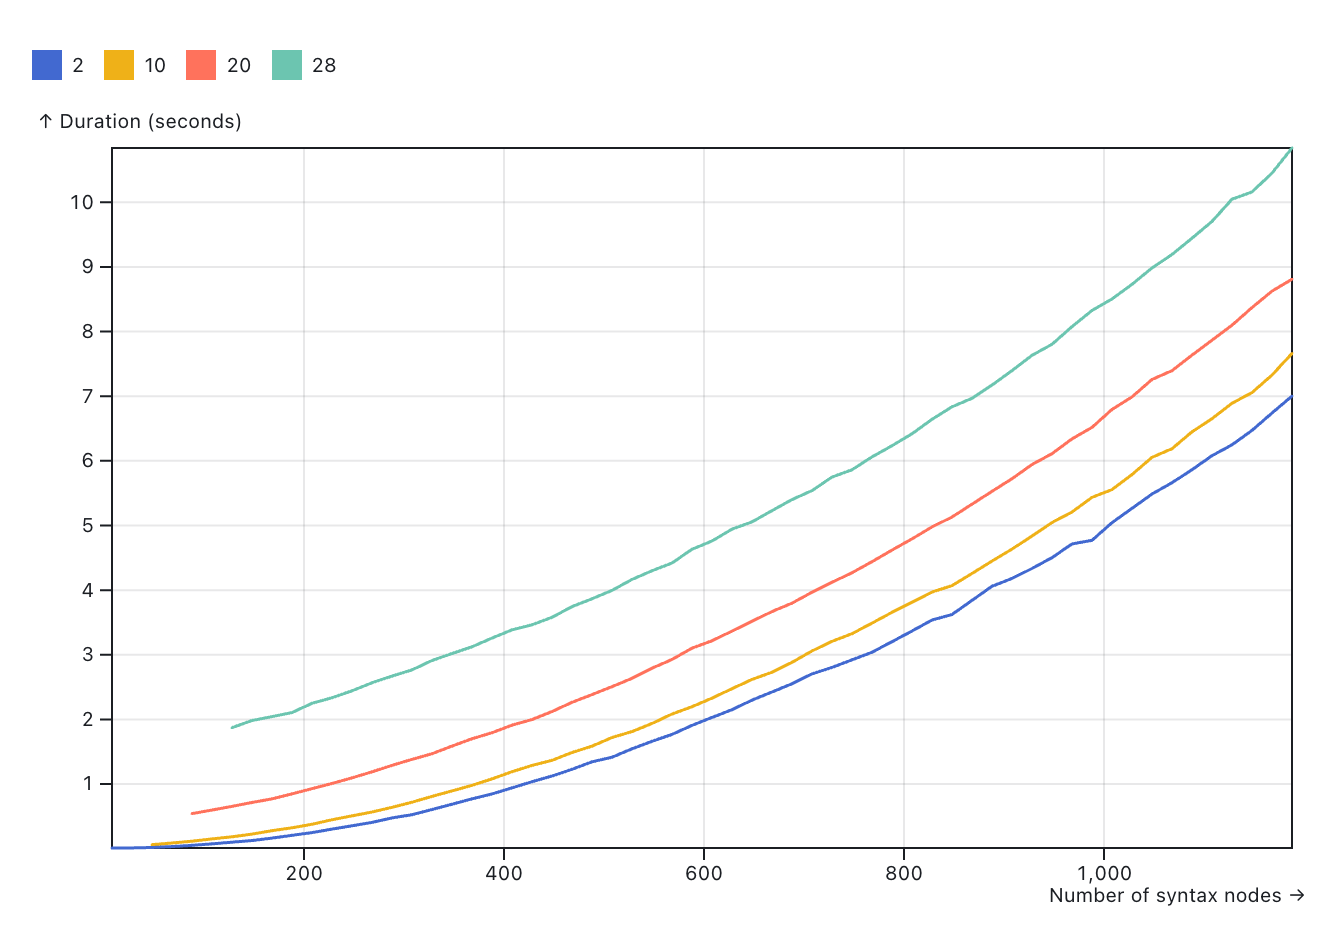
\includegraphics[width=0.8\linewidth]{images/program-size.png}
    \caption{Performance by Program Size, Measured in Syntax Nodes}
    \label{fig:node-size}
\end{figure}

It is worth clarifying that performance bottlenecks are largely due to MUS enumeration rather than parsing or static analysis, as these processes are negligible for reasonably sized programs. Also note that other files in the projects that are not being currently inspected and 3rd party library files do not contribute to the computation cost of MUS. Those files are translated into constraints, but are considered as assumptions, and do not participate in the shink process.

\paragraph{Multi-step Type Errors}

To better understand the effect of multi-step type error on performance, we generated a series of defective programs, each one containing a multi-step type error. These programs vary in 2 dimensions: the size of the program, ranging from 4 syntax nodes to 1000 syntax nodes, and the number of steps in the type error, ranging from 2 to 30. In this way we can compare the performance on the set of programs who are similar in length but contain type errors involve different number of steps. Fig.~\ref{fig:multi-step-time} plots how 5 of these sets.  It can be seen that the impact of program size is independent from the impact of the number of steps in the errors. For a program with 200 syntax nodes, it takes 0.275 seconds to diagnose; with 30 steps, it requires 2.8 seconds. While for the program with 1000 syntax nodes, 2-step errors takes 5 senconds and 30-step errors take 9 seconds.

\begin{figure}[ht]
    \centering
    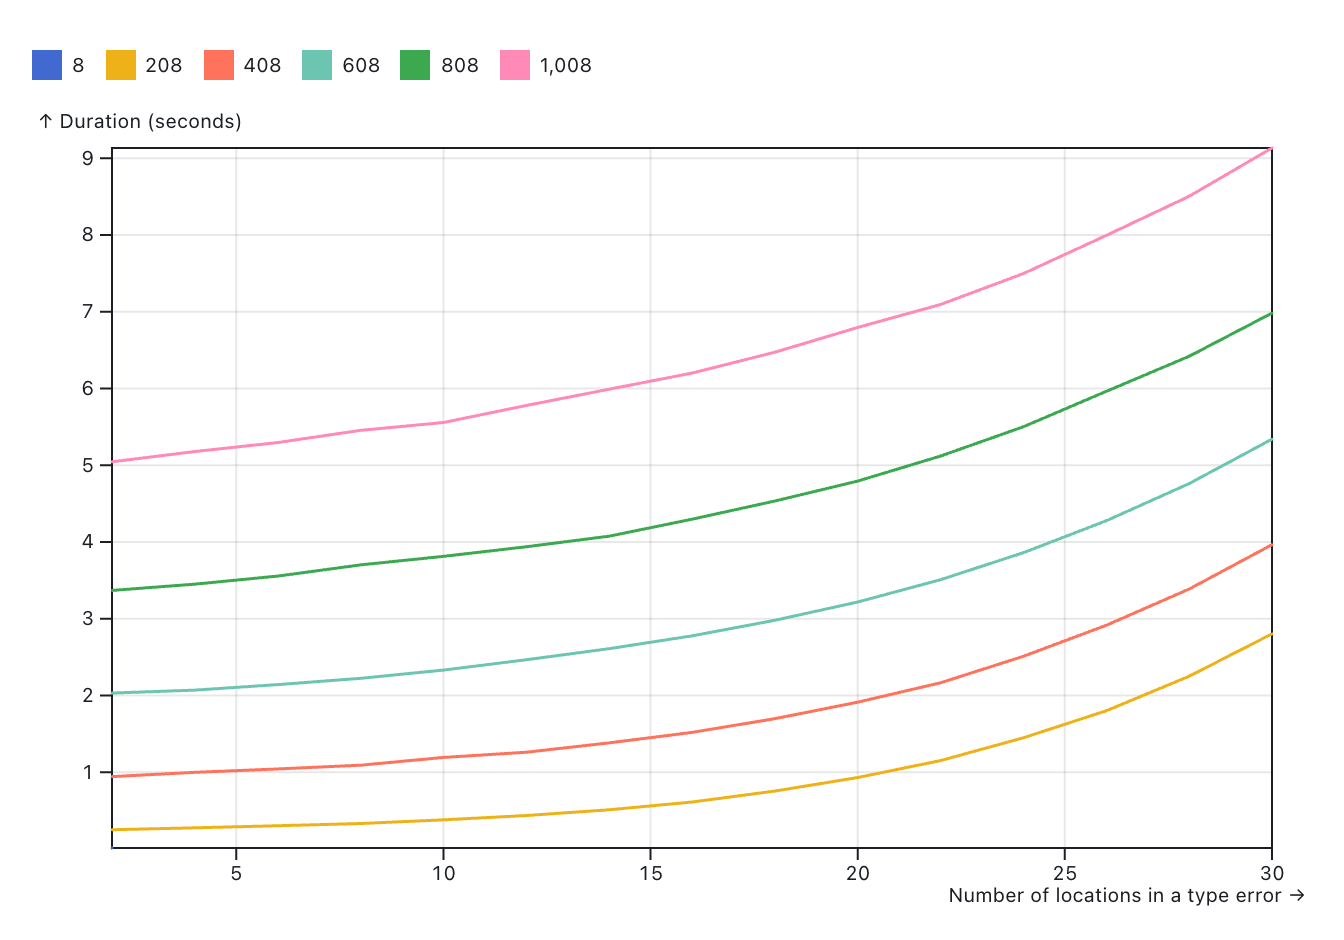
\includegraphics[width=0.8\linewidth]{images/multi-step.png}
    \caption{Multi-step Type Error Impact on Performance}
    \label{fig:multi-step-time}
\end{figure}

\paragraph{Multi-witness Type Errors}

Similarly we generated multi-witness type errors that vary in length (4 to 1200) and the number of witnesses (2 - 30) on one side of typing conflict. These errors were generated using the form \lstinline{x y = case y of 1 -> 1; '2' -> 2; '3' -> 3}. With 30 error locations and 200 syntax nodes, diagnosis takes a similar time as multi-step errors. With 1000 syntax nodes, it takes over 43.68 seconds (Fig.~\ref{fig:multi-witness-time}).  We can visually identify the linear growth in computation time, that is because we only increase the number of witness on one side. Recall that for a type error involves $m$ witnesses on one side and $n$ on the other, there will be a total of $m \times n$ MUSes.

\begin{figure}[ht]
    \centering
    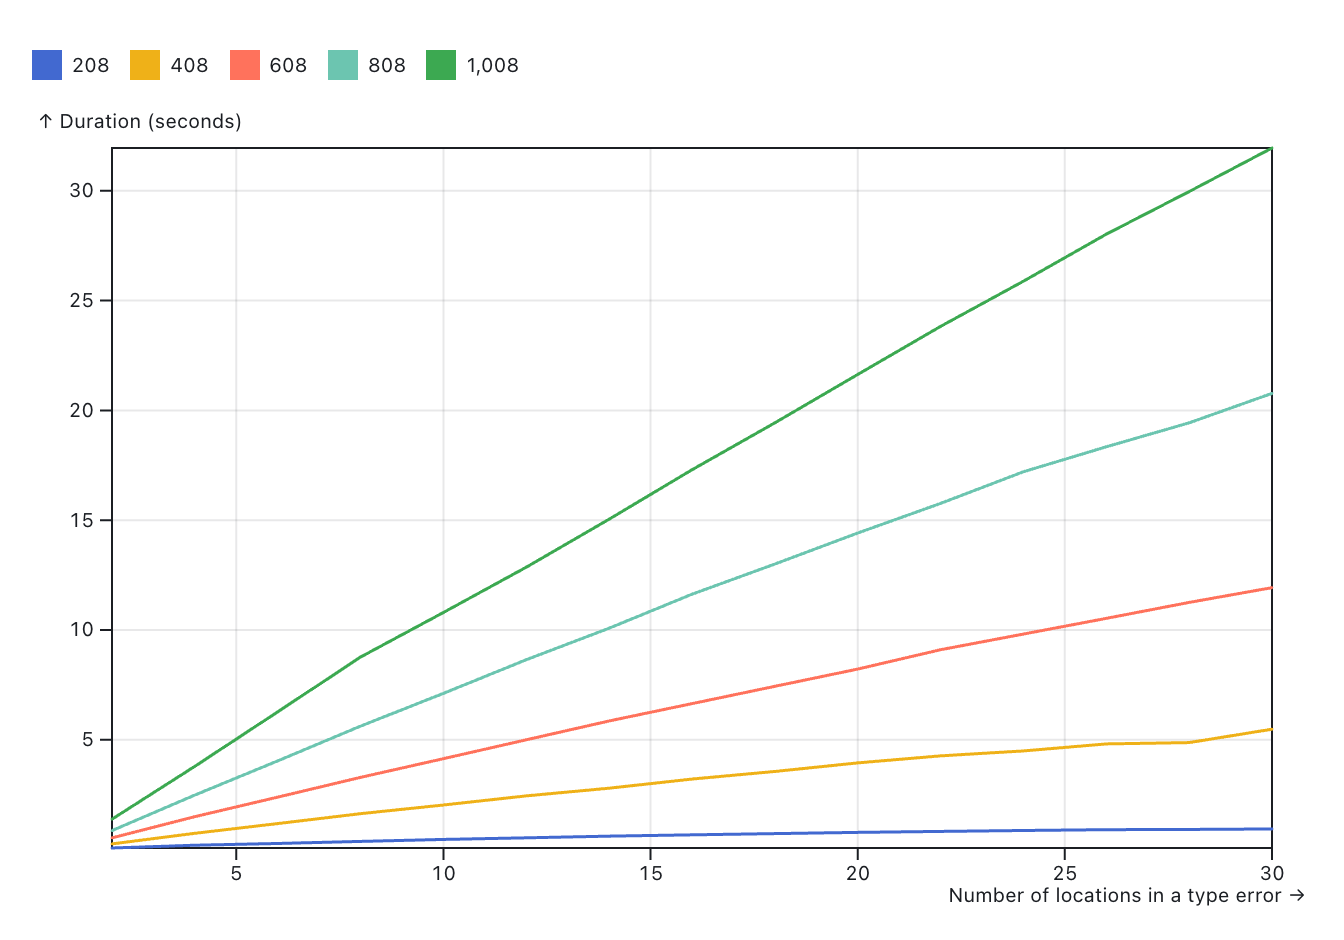
\includegraphics[width=0.8\linewidth]{images/multi-witness-time.png}
    \caption{Multi-witness Type Error Impact on Performance}
    \label{fig:multi-witness-time}
\end{figure}

\paragraph{Multi-party Type Errors}

Multi-party type errors, are often multiple simple errors fused into one, and are the most computationally intensive. Again, we generated programs varies in length (from 5 nodes to 1200 node) and the number of parties (from 3 to 30 parties). To note that this experiment does not mean to be representative of realistic type error. It is highly unlikely to have more than a 3 parties in real world programming, for more than that, programmers have to ignore an existing type error and continue adding more ill-typed code fragments. Our results (Fig.~\ref{fig:multi-party-time}) shwo that, for 30 error locations and 200 syntax nodes, diagnosis requires 3.15 seconds; with 1000 nodes, it takes over two minutes. Recall that for a multi-party type error with $n$ parties, then there are $n (n - 1) / 2$ unique MUSes. The growth pattern in computation time roughly reflect this correlation.

\begin{lstlisting}[language=Haskell, caption=Multi-party Haskell Example, label={lst:eval-multi-party}]
data X = X
data Y = Y
data Z = Z
f a = case a of
  X -> 1
  Y -> 2
  Z -> 3
\end{lstlisting}

\begin{figure}[ht]
    \centering
    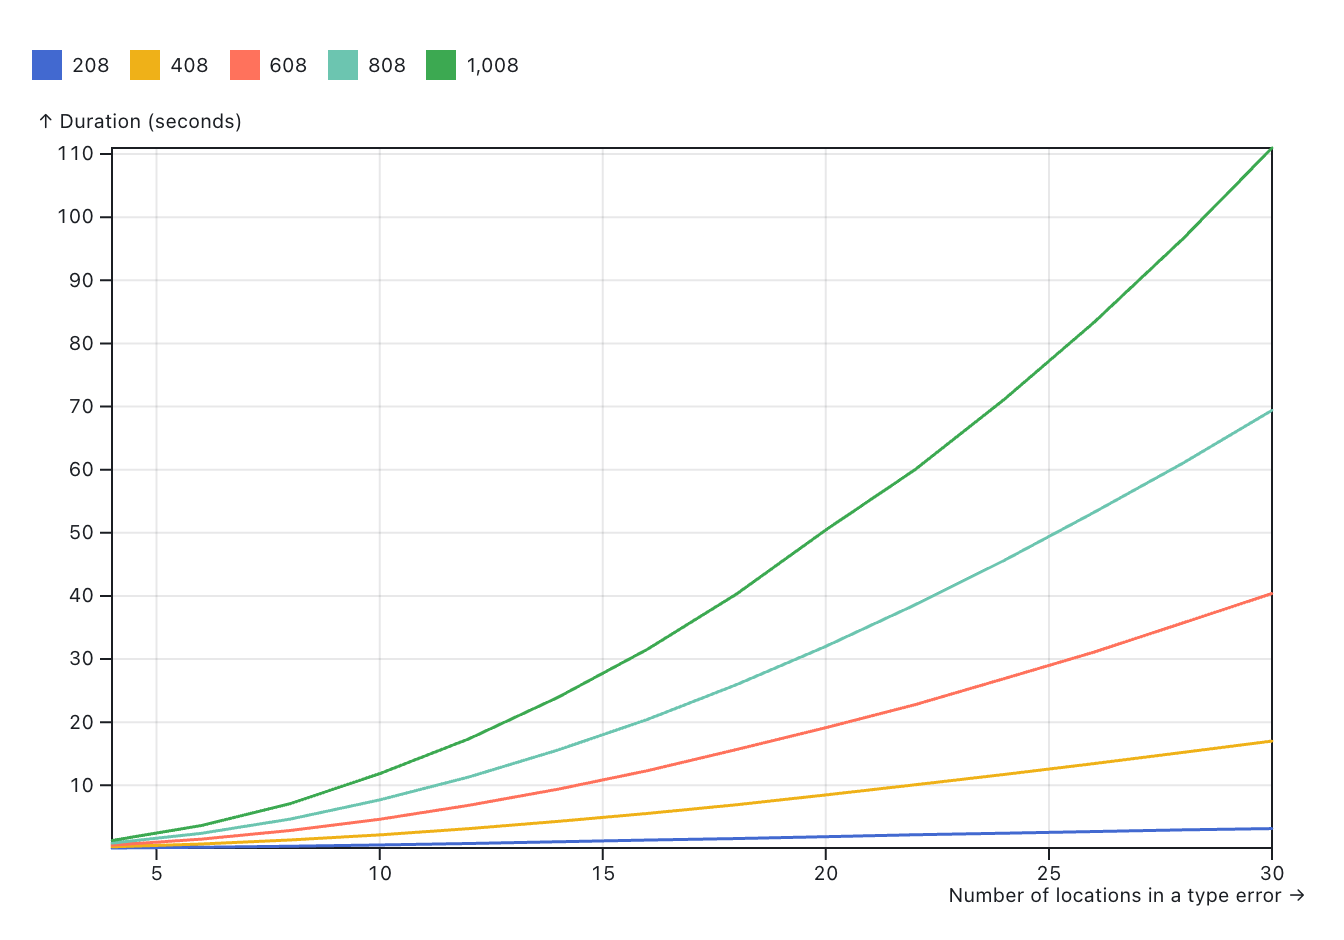
\includegraphics[width=0.8\linewidth]{images/multi-party-time.png}
    \caption{Multi-party Type Error Impact on Performance}
    \label{fig:multi-party-time}
\end{figure}

\paragraph{Performance Summary}
The size of program impact the performance of Goanna, so does the category of errors and how complex they are. In short, multi-party errors present the most significant computational challenge among the categories, followed by multi-witness and multi-step errors (Fig.~\ref{fig:compare-time}). This performance constraint roughly corresponds with the number of MUSes present in the type error. 

\begin{figure}[ht]
    \centering
    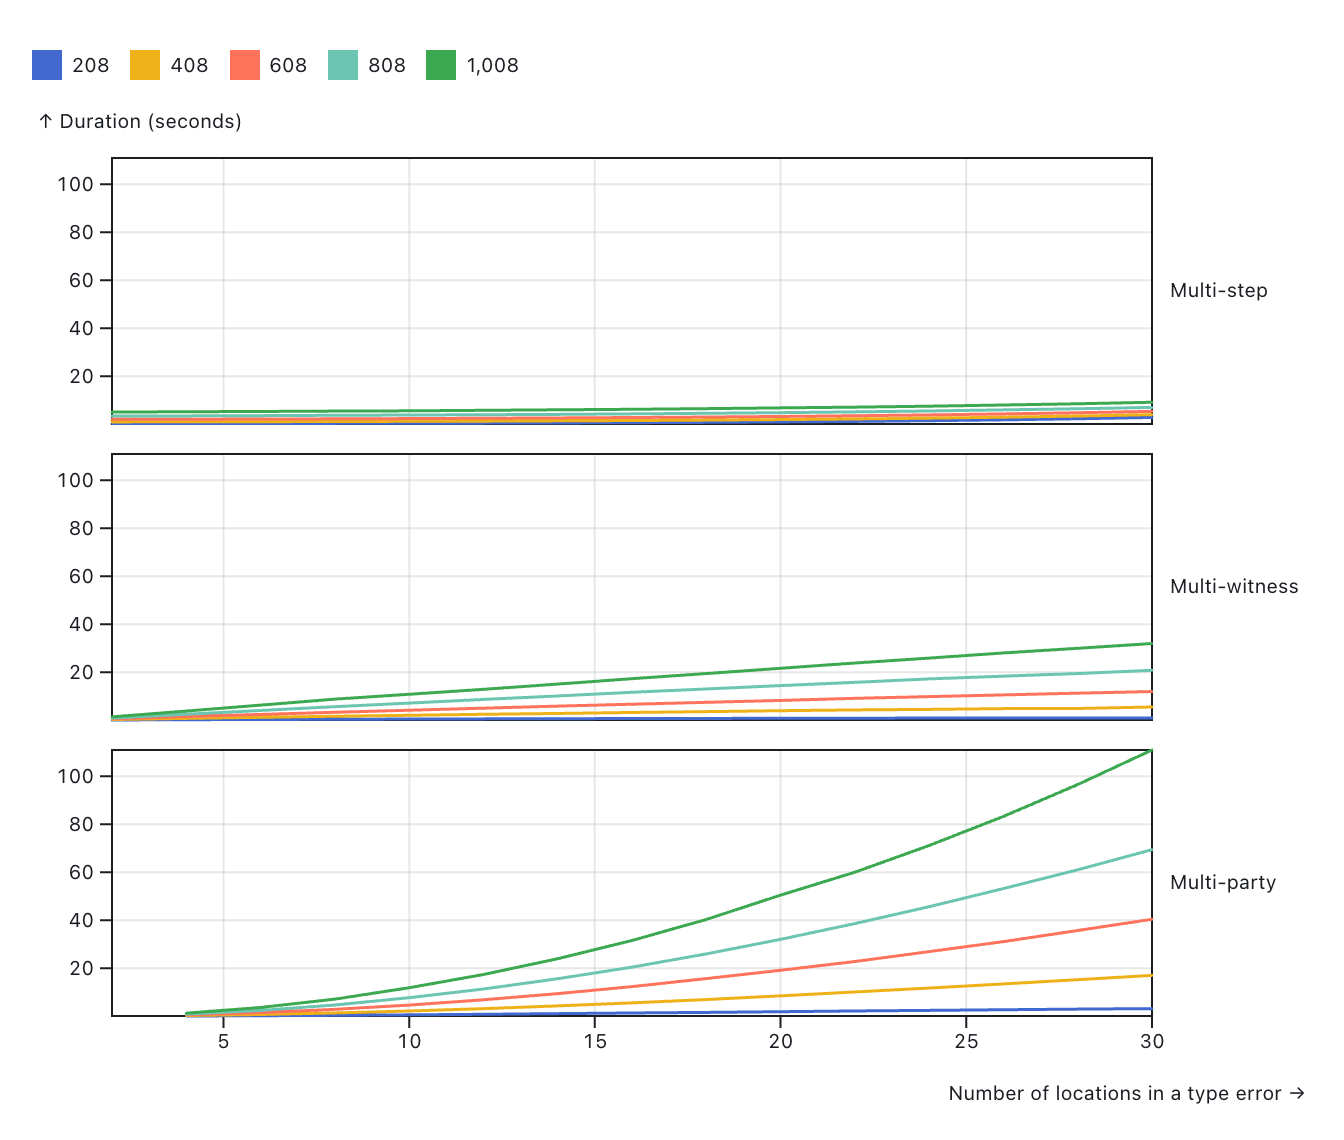
\includegraphics[width=\linewidth]{images/compare-time.png}
    \caption{Comparison of Performance Across Error Types}
    \label{fig:compare-time}
\end{figure}


\section{Discussion} \label{sec:discussion}

This section begins with an examination of Goanna's accuracy and reliability, along with its practical advantages over traditional tools. We then analyze the trade-offs made in Goanna's performance and explore potential improvements. Finally, we compare the strengths and weaknesses of Goanna with Large Language Model (LLM)-based programming assistance and explore how these two approaches can be integrated for optimal benefits.

\subsection{Strengths of Goanna and MCS-based Error Diagnostics}

Goanna is the first debugging tool to use Minimal Correction Subsets (MCS). In comparison to traditional methods like Hindley-Milner and constraint-based type inference using Minimal Unsatisfiable Subsets (MUS), Goanna provides a more concise cause analysis and better guesses of root causes. It identifies all type errors in the source file rather than just one and infers the most concrete types for the entire source program.

\paragraph{Remove Biases in Type Error Reporting}

One factor that Goanna surpasses traditional tools in accuracy is due to its unbiased approach toward all possible causes. Conventional compilers and type checkers such as GHC and Helium, terminate upon finding the first type error, result in only the usage of a function is reported in the error message, its definition was never blamed, an issue known as left-to-right bias in traditional type-checking algorithms, a notable shortcoming that limits the usability of error messages \cite{McAdam2002-vb, Lee1998-fx, Chen2014-ev}. 

Unlike conventional compilers which add constraint one at a time, Goanna applies a holistic approach, colloquially known as ``the French method'', by collecting all constraints from the source program and delaying the solving until the entire program has been translated into a constraint-level intermediate representation. This approach allows Goanna to asserting multiple assumptions regarding the type error using constraint programming techniques. In practice, reporting multiple possibilities for an error is highly useful. Programmers are equally prone to making mistakes in both calling and defining functions. It has been noted that some common causes of type errors among Haskell programmers occur at the definition site, such as outdated type annotations.

\paragraph{Meaningful and Familiar Idioms to Better Understand Type Errors}

Goanna uses MCS as the building block of a type error diagnosis. This choice allows type errors to be presented as a list of possible causes, each cause shows a smallest set of changes required to fully resolve the error. Goanna is not unique in employing this paradigm of debugging errors. This type of error diagnosis has been utilized in various user interface designs such as autocorrect software. Additionally, Goanna allows programmers to preview each possible cause: when navigating to a cause, locations need to be changed are highlighted, the effect of these changes on the program semantics and types are reflected through dynamically updated type hints. This interface idiom is analoguous to how merge conflict resolution tools in mordern version control systems.

\paragraph{Full Type Hints on ill-typed Program}

In statically typed languages, particularly those like Haskell  expressions are implicitly typed (type annotations are optional), understanding the types of various expressions is integral part of making sense of the program. Traditional approaches, such as \texttt{:t expression} command in GHCI, run in interactive shells or command lines. Modern editors enhance this functionality by providing text overlays for instant type overview \todo{example}. However, these type hints are available only when the program is well-typed; they either become unavailable or outdated when type errors occur. This limits their usefulness, as they are much more in need during resolving type errors.

Goanna addresses this issue by inferring types for ill-typed programs to the greatest possible extent using the Maximal Satisfiable Subset (MSS). MSSes are the complement set to MCS, therefore, Goanna has access to an MSS to each MCS. The intuitive is that MSS represents the largest portion of the source code that is well-typed, allowing a set of  type assignments for each possible cause. That is, Goanna's type hints are two-dimensional: they encompass every expression in the program and also reflect how types would change if a different cause for type error is selected. This additional information helps verify whether a Goanna's diagnosis aligns with the programmer's true intentions, providing more confidence in identifying the root cause.

\subsection{Optimizing Performance}

As we preluded in Section \ref{sec:evaluation}, Goanna's  performance is constraint by the computational cost of the MUS enumeration. More specifically, the performance is limited by the efficiency in discovering a single MUS through the shrink algorithm and the total number MUSes present in the program. 

To eliminate the first limitation, one potential solution is to segment the number of constraints of an entire file into smaller chunks, such as top-level function definitions, and process these sequentially in topological order or in parallel. Goanna chose to use a single file as the smallest type checking unit to provide a concise and minimal formalization of constraint based type system.  Smaller sized source code units results in smaller constraint system, which in turn would  improve the performance profoundly. This method is similar to how mainstream compiler tools manage type checking in real world programs. 

To address the second limitation, a feasible approach is to explore different MUS enumeration algorithms. The parallel capabilities of advanced MUS enumeration methods \cite{Zhao2016-bu, Bendik2020-pz} have not been fully explored in this study. In addition, partial MUS enumeration \cite{Previti2013-mr, Liffiton2016-xi} can be employed, to provide early results to the programmer instead of waiting for the complete list of possible causes.


\subsection{Comparison with Large Language Models} \label{sec:llm}
    
LLMs were actively experimented with performing programming related tasks such as wirting code, finding logical errors and generating documentations.  This development is tangential to Goanna's objectives of explaining type errors and supporting easier resolution of type errors. 

\begin{figure}[hbt]
  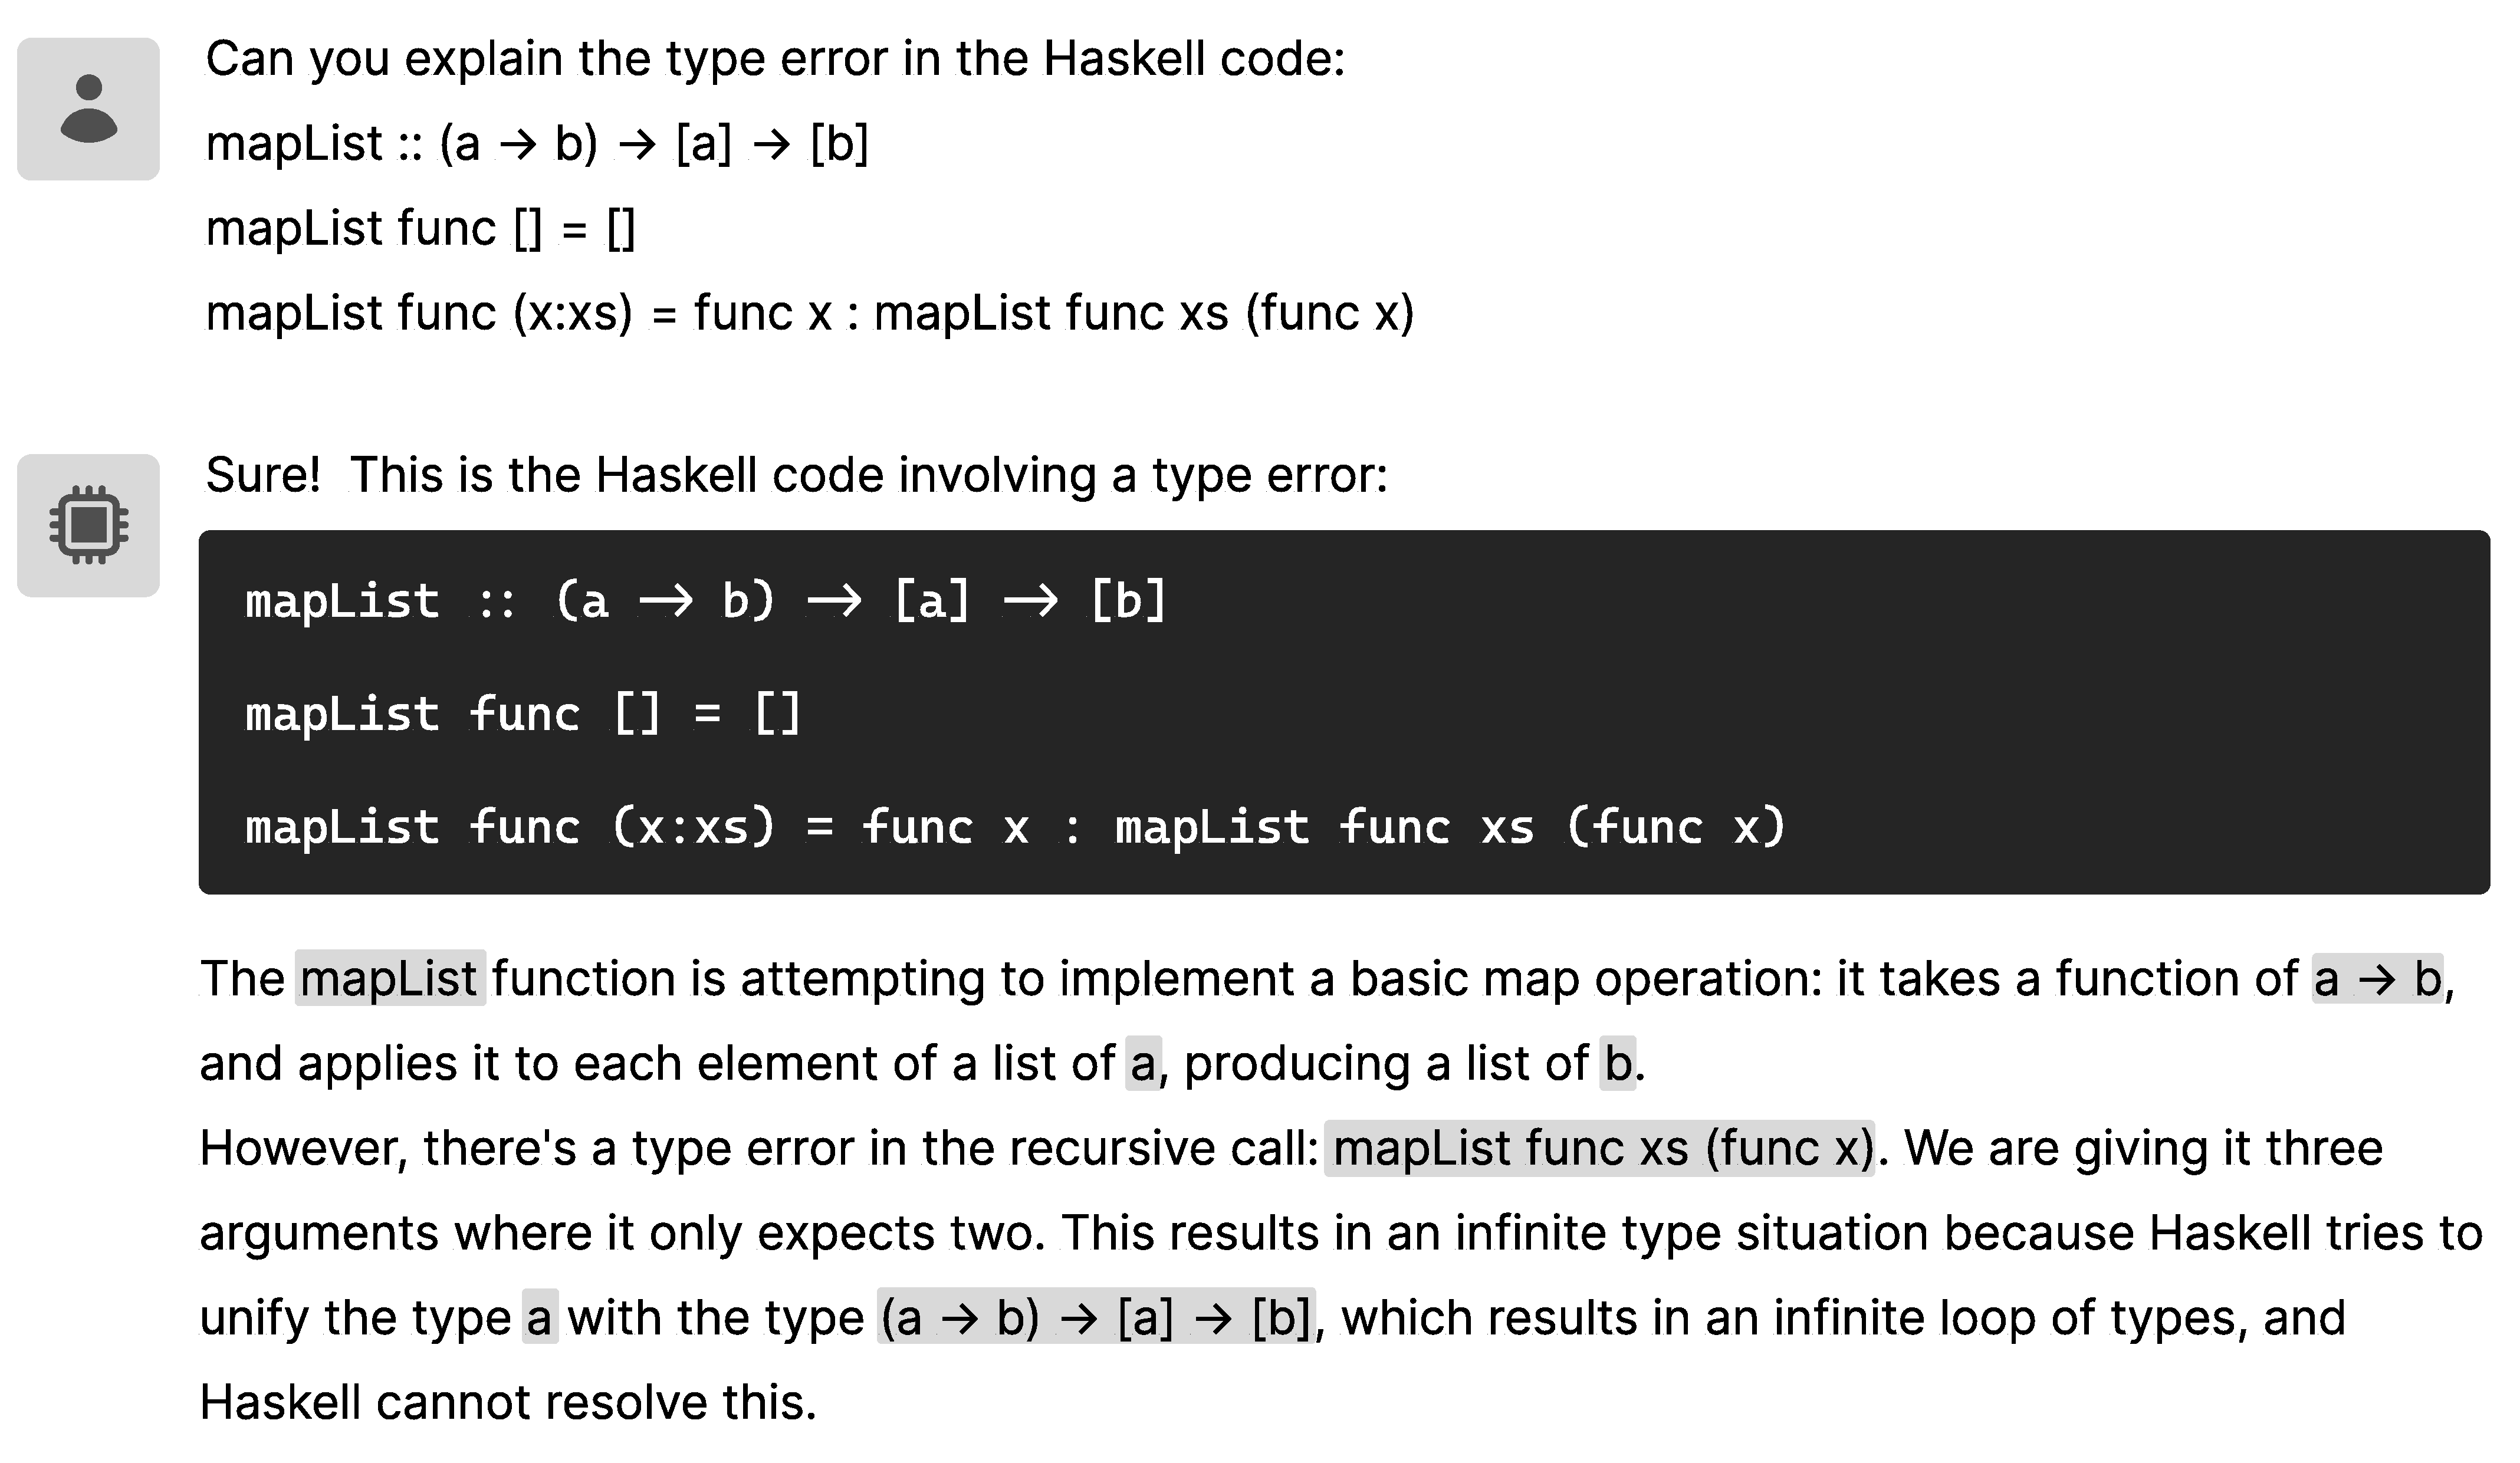
\includegraphics[width=\linewidth]{images/LLM.pdf}
  \caption[LLM explaining a type error; it began very accurate, then went on to give incorrect and contradicting analysis]{\label{fig:llm}
  The figure shows the user prompted LLM to explain the type error in a Haskell function definition \texttt{mapList}. LLM, at first, showed a profound understanding of the subject matter, clearly explained the intention of the function, and accurately identified the error location. In the last sentence, LLM claimed the definition would result in an infinite type because trying to unify \texttt{a} with \texttt{(a -> b) -> [a] -> [b]}. In reality, unifying two functions with different numbers of arguments will not cause infinite types. 
    }
\end{figure}

While LLMs have shown capability in recognizing basic errors, they often display a limited understanding of type theories and reasoning ability. Fig.~\ref{fig:llm} depicts a type error caused by mismatching numbers of arguments in the function \texttt{mapList}; although provided a correct error identification at the start, GPT 4 proceeded to claim, “This results in an infinite type situation because Haskell tries to unify the type \texttt{a} with the type \texttt{(a -> b) -> [a] -> [b]}, which results in an infinite loop of types, and Haskell cannot resolve this,” illustrating a fundamental lack of understanding of type theory.

\begin{figure}[hbt]
  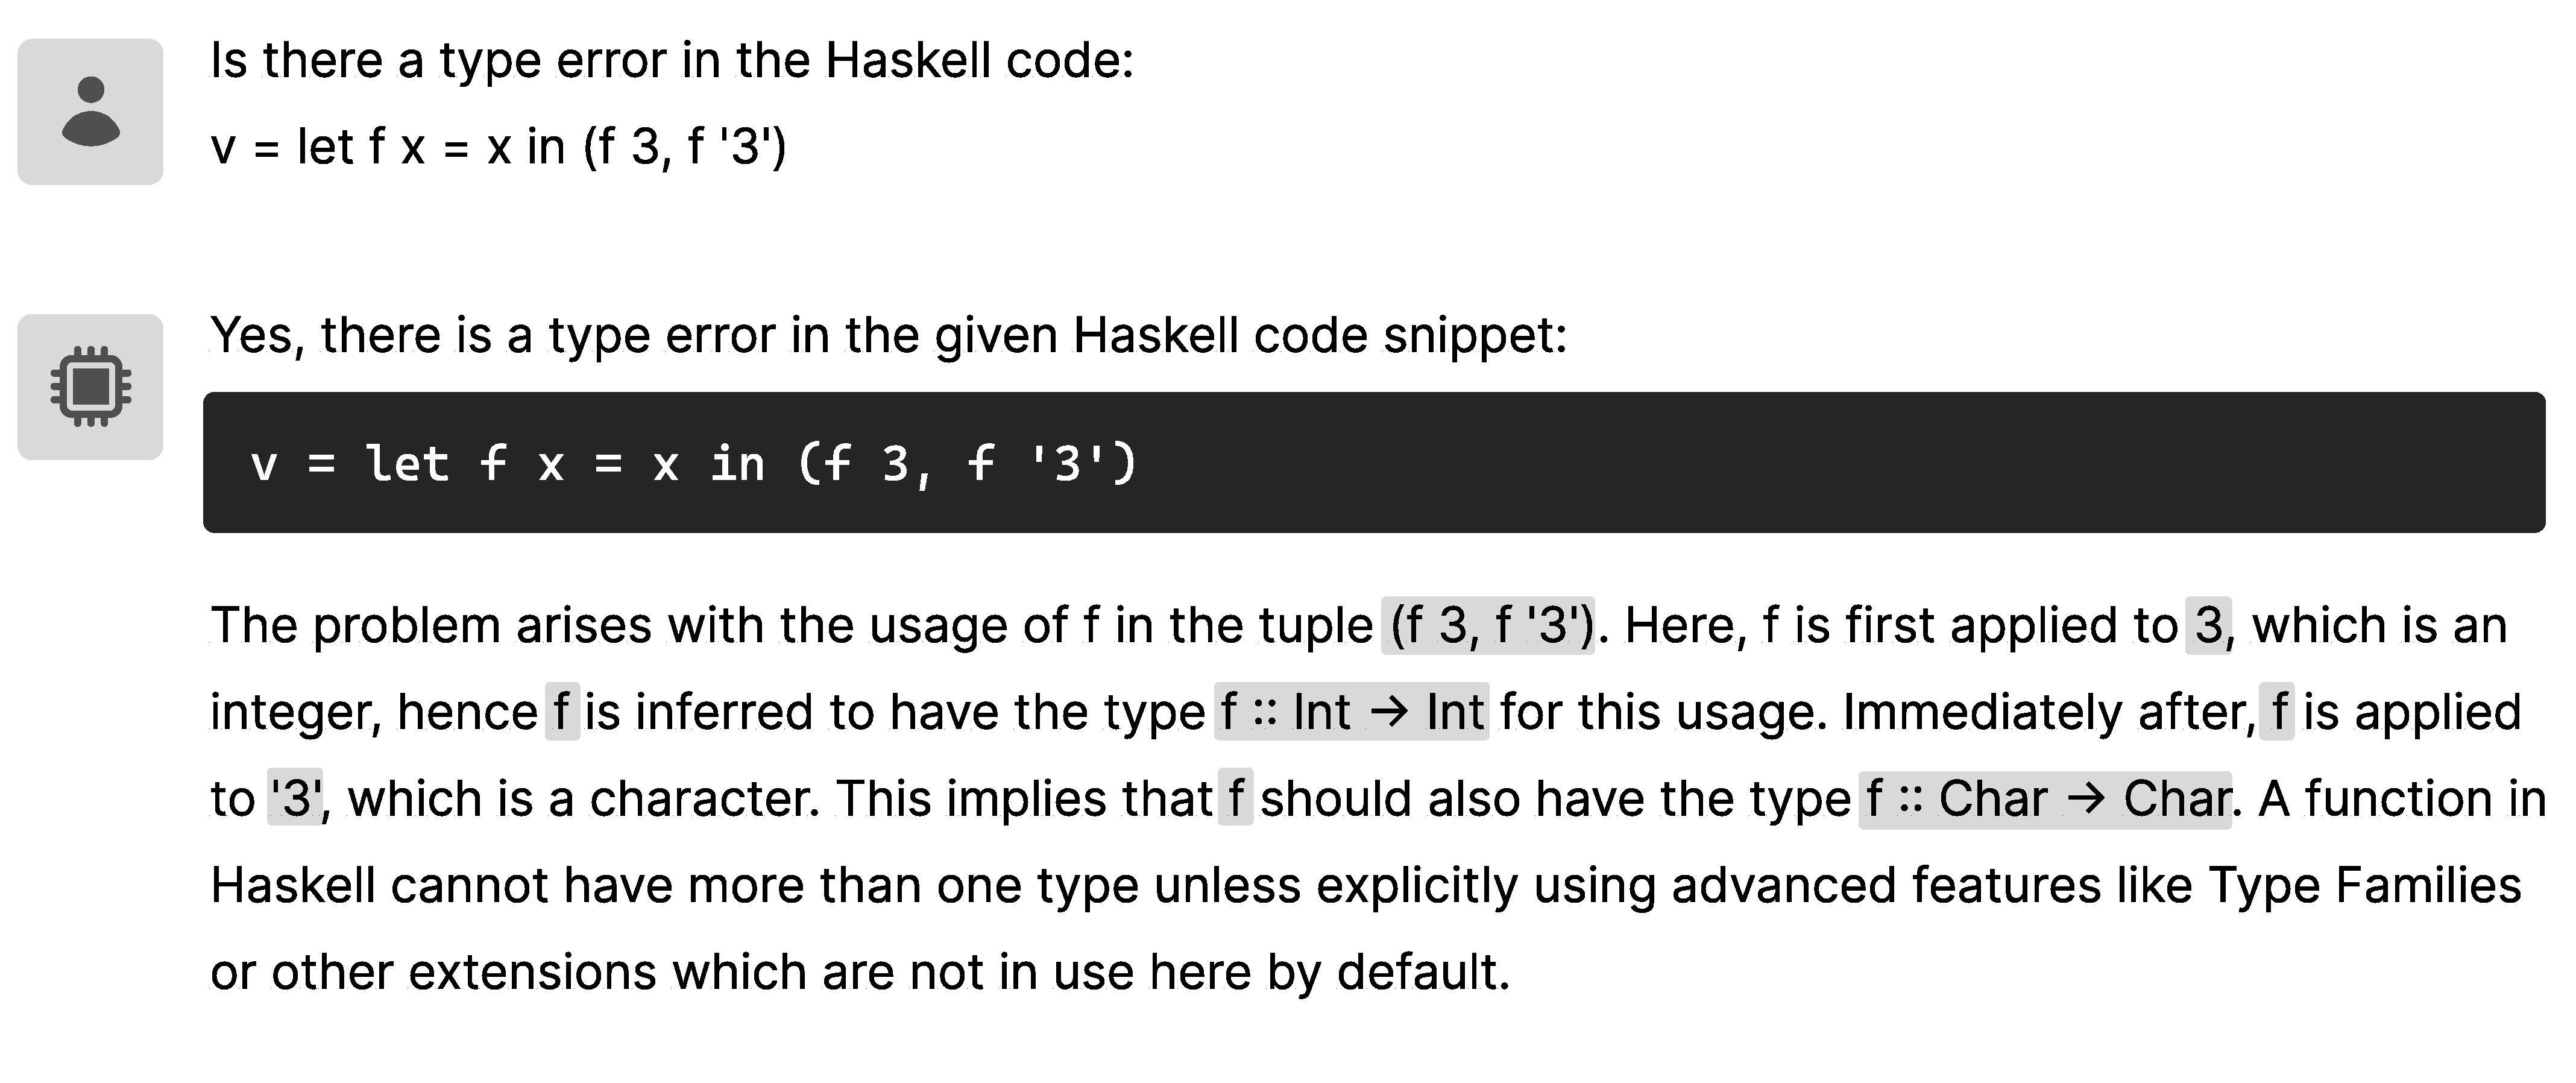
\includegraphics[width=\linewidth]{images/LLM2.pdf}
  \caption[An example where LLM identified a type error in well-typed source code]{\label{fig:llm2}
  The figure shows a user asking an LLM whether the provided Haskell source code has a type error. While the provided code is, in fact, well-typed, LLM hallucinated a type error and ignored how polymorphic functions work in Haskell. In the example, the function \texttt{f},  defined the same way as the \texttt{id} function, can be applied with a value of any type.
    } 
\end{figure}

When tested with the prompt "Is there a type error in the Haskell code: v = let f x = x in (f 3, f '3')", most LLMs incorrectly reported yes (Fig.~\ref{fig:llm2}). However, this Haskell code is indeed well-typed. LLMs can give wrong explanations and find type errors that do not exist, unlike tools like GHC, Helium, and Goanna. While there is clearly a role for their usage in programming assistance \cite{Lee2024-hs}, they do not “reason” about types and, hence, are not trustworthy.

While LLMs are getting more and more accurate with each iteration, some doubt whether they will ever become as reliable as theory-based tools \cite{Berglund2023-ig}. We believe in the great potential of integrating LLMs with existing theory-based tools, such as Goanna. This integration could enhance the performance of LLMs by aligning their operations with accurate theoretical guides or utilizing their strengths to complement traditional tools' shortcomings, such as suggesting syntactical improvements, and coming up with personalized error message suited for the programmers skill level. This synergy could lead to more robust programming assistance using both types of tools. We propose two candidate workflows:

\itemize{
  \item{\textbf{Code Generation with Validation}: LLMs could generate initial source code based on user-provided prompts. Theory-based tools, such as Goanna, then check for errors. Detected errors could be fed back to the LLMs for corrections, enhancing both the efficiency and accuracy of code development.}
  \item {\textbf{Error Tutoring and Resolution}: Theory-based tools could identify errors in manually written code, with LLMs suggesting syntax corrections. This combines the precise error detection from traditional theory-based tools with the ability of LLMs to generate effective syntax changes, surpassing traditional tools in this domain.}
}

\section{Related Work} 
    \label{sec:related-work}
    In this section, we survey the corpus of work that Goanna built upon and was inspired by. We first review the work that is built on a theoretical foundation similar to that of Goanna. We then examine studies that share similar aims and offer a debugging experience comparable to Goanna's. Finally, we delve into research on program slicing and discuss how Goanna extends the concept of slicing and distinguishing itself from its predecessors.

    \subsection{MCS enumeration}
	
    MCS enumeration has been extensively studied in the field of error localization across various domains. MCS is used to optimize package management system \cite{Ignatiev2014-nr} and to explain decisions made by machine learning algorithms \cite{Marques-Silva2023-nk}.
    
    
    In the specific context of type error diagnosis and resolution, several related approaches have been explored. It is important to examine the strengths and weaknesses of Goanna in the context of these areas.

    One notable work by Lamraoui et al. introduced a tool \cite{Lamraoui2016-wr} that utilizes the capability of MCS to localize multiple faults and identify software defects using unit tests. Their approach demonstrated the effectiveness of MCS in pinpointing errors within a program. Similarly, Bekkouche et al. conducted a relevant study  \cite{Bekkouche2015-is}  on MCS utilization for locating program errors in while-loop programs. Their findings showed improved efficiency compared to SAT-based approaches. Although showing strength in programming language static analysis, MCS-based fault localization has not been previously applied at the type system level. Goanna distinguishes itself as the first tool to explore this approach within the realm of type error diagnosis and resolution.

    \subsection{Suggesting changes to type errors}
   Lerner et al. proposed Seminal \cite{Lerner2007-mu}, using syntax mutation and binary search to find appropriate syntax changes to program errors. The advantage of Seminal is that it's capable of suggesting direct syntax changes to common mistakes (e.g., mistakingly swapping the order of function arguments). However, it is impossible for Seminal to provide the complete set of all potential fixes. Nor does it guarantee a suggested solution is minimal syntax change.
   
   Counter-factual typing (CFT) \cite{Chen2014-dz,Chen2020-ad} uses a variation-based type system; it is capable of suggesting the correct type for all possible. CFT shares many capabilities with Goanna, CFT is able to suggest multiple-location changes, CFT uses similar ranking heuristics. Goanna is able to produce an in-depth analysis of the ill-type program, such as type error isolation. CFT and Goanna both aim to produce a complete set of potential fixes, Goanna employs a set of effective algorithms to reduce the exponential number of potential fixes without reducing the quality of suggestions. 
   
   SHErrLoc \cite{Zhang2015-xy} uses constraints as the underlying to perform type inference and type error diagnoses. SHErrLoc is able to suggest multiple possible fixes of the type error and rank them based on heuristics. Unlike Goanna's approach of using a general-purpose constraint language, SHErrLoc relies on GHC's internal constraints and then translates them into SCL (a custom-made constraint language). On the technical side, this approach relies heavily on modification of the compiler and does not remain reliable with later GHCs. Most importantly, there is no way to interact directly with the solver. This renders the kind of constraint manipulation in Goanna and SHErrLoc impossible. Goanna is able to perform type reconstruction for ill-typed programs, that is, finding the most concrete types for all expressions for each potential solution using the Maximal Satisfiable Subsets. SHErrLoc focuses on finding the locations only.


\subsection{Type Error Slicing}

Type error slicing \cite{Haack2004-fr} is a technique to identify all necessary locations of a type error that is necessary for programmers to diagnose the root cause. It has been studied in many studies ever since \cite{Tip2001-qn, Heeren2003-kd}. These studies all use Minimal Unsatisfiable Subset (MUS) to ensure the \textit{completeness} and \textit{minimality}. The drawback of type error slicing is that it often produces too many locations.  Chameleon \cite{Stuckey2003-pz,Fu2021-xd} improved type error slicing by allowing programmers to interactively show the partial MUS by choosing their own assumptions. Compared to these tools that base their analysis on a single MUS, Goanna effectively utilizes all possible MUSes. This allows Goanna to enhance its suggestions based on the improved knowledge of the underlying type of error. For example, it uses the number of MUSes a location appears in to rank how likely the location is part of the root cause. This is not possible with a single MUS.  

\section{Future Work}\label{sec:future-work}

\subsection{Planned User Studies and Research Questions}

Our evaluation for Goanna so fare relies on existing datasets and program generation. Evaluating Goanna with human participants is crucial for obtaining qualitative insights into its usefulness in providing explanation and supporting sense making in complex type errors. We have coducted a few preliminary workshop studies, participants exhibited positive reactions when using Goanna. However, a rigorous human study based on realistic debugging use cases is planned for the near future. We aim to investigate the following questions:

\itemize{
  \item Can Goanna's accuracy in type error identification contribute to improved understanding and performance in real-world programming tasks?
  \item Which user interface paradigms effectively leverage Goanna's strengths (such as accessing all possible error causes) and mitigate its limitations (such as slow response times with large programs)?
}

\subsection{Suggesting Syntax Approaches}

Goanna's suggestion is limited by the fact that it only provide type level suggestions. For example, it may suggest {\it change this string literal ``3'' to an expression of type Int}, but not {\it change this string literal ``3'' to 3}.  An exciting avenue for enhancement its ability to suggest syntax changes that potentially solve the type error. As noted in \cite{Chen2014-dz}, syntax changes pose significant challenges. However, with recent advancements in generative models and research progress in ML-based type error resolution \cite{Seidel2017-uf}, the development of accurate syntax change suggestions is becoming increasingly feasible, as we discussed in Section \ref{sec:llm}.

\subsection{Supporting Additional Languages}

Expanding Goanna's capabilities to encompass other functional programming languages beyond Haskell is also a consideration. Languages such as Scala and OCaml, which practice similar type system to Haskell, can directly benefit from Goanna's functionalities. We also intend to extend these techniques to popular multi-paradigm languages such as TypeScript and Rust in the future.



\section{Summary} \label{sec:conclusion}

In this paper, we introduced Goanna, a tool for identifying and resolving type errors in Haskell code, and Goanna-IDE, a interactive programming environment for Haskell. We demonstrated the features of Goanna through examples, including its fix suggestions, type error grouping, and identifying multiple type errors. We also discussed our approaches to reduce and reprioritize potential causes.

We evaluated the effectiveness of Goanna from a set of 153 Haskell programs from online sources and research papers and demonstrated its ability to identify the root causes type errors accurately and reliably compared to other tools. We also evaluated Goanna's performance in controled benchmarks. We show that Goanna perform well against small to median sized program. Goanna currently works with Haskell, but in the future, we plan to extend its MCS-based error diagnosis to work with other strongly typed languages.


\bibliography{paperpile}

\end{document}


    % \subsection{Threats to Validity}

    % \paragraph{\textbf{Selection of the dataset}}
    % Our selection of dataset is limited in its number. This is due to the challenge of finding programs that contain type errors. Unlike runtime errors, which can be mined from code repositories and version control histories, type errors in Haskell can be detected by the compiler tool, and ill-typed programs are usually fixed before the changes are committed to the version control systems. Further, we employed two selection methods. First, the error is indeed a type error. We test this by running the original program in GHC and checking if it indeed triggers a type error. The program is discarded otherwise, for instance, if it contains only parsing errors or runtime errors. Second, we discarded type questions where the main error relies on third-party libraries. 
    
  
        
    % \paragraph{\textbf{Measurement of performance}} Performance on Goanna and GHC was measured on a Linux virtual machine with a 3.1 GHz Processor and 2GB RAM. In practice, complex systems like this may perform differently depending on hardware and software configurations. Although we were not able to extract the performance profile of each tool across different platforms and operating systems, we chose hardware with abundant resources and up-to-date software dependencies. During our performance measuring, neither CPU usage nor memory usage was fully stressed. Additionally, GHC was run with the ``-fno-code'' flag enabled to limit its usage to type-check only.



